\documentclass{ximera}

\begin{document}
	\author{Stitz-Zeager}
	\xmtitle{TITLE}


\mfpicnumber{1}

\opengraphsfile{ExponentialEquationsandInequalities}

\setcounter{footnote}{0}

\label{ExponentialEquationsandInequalities}

In this section we will develop techniques for solving equations involving exponential functions.  Consider the equation $2^{x} = 128$.  After a moment's calculation, we find $128 = 2^{7}$, so we have $2^{x} = 2^{7}$.  The one-to-one property of exponential functions, detailed in Theorem \ref{explogsonetoone}, tells us that $2^{x} = 2^{7}$ if and only if $x=7$.  This means that not only is $x=7$ a solution to $2^{x} = 2^{7}$, it is the \textit{only} solution.  

\smallskip

Now suppose we change the problem ever so slightly to $2^{x} = 129$.  We could use one of the inverse properties of exponentials and logarithms listed in Theorem \ref{invpropslogs} to write $129 = 2^{\log_{2}(129)}$.  We'd then have $2^{x} = 2^{\log_{2}(129)}$, which means our solution is $x = \log_{2}(129)$. 

\smallskip

After all, the definition of $\log_{2}(129)$ is `the exponent we put on $2$ to get $129$.' Indeed we could have obtained this solution directly by rewriting the equation $2^{x} = 129$ in its logarithmic form $\log_{2}(129) = x$.  Either way, in order to get a reasonable decimal approximation to this number, we'd use the change of base formula, Theorem \ref{changeofbase}, to give us something more calculator friendly.  Typically this means we convert our answer to base 10 or base $e$, and we choose the latter: $\log_{2}(129) = \frac{\ln(129)}{\ln(2)} \approx 7.011$.  

\smallskip

Still another way to obtain this answer is to `take the natural log' of both sides of the equation. Since $f(x) = \ln(x)$ is a \textit{function}, as long as two quantities are equal, their natural logs are equal.\footnote{This is also the `if' part of the statement $\log_{b}(u) = \log_{b}(w)$ if and only if $u=w$ in Theorem \ref{explogsonetoone}.} 

\smallskip

We then use the Power Rule to write the exponent $x$ as a factor then divide both sides by the constant $\ln(2)$ to obtain our answer.\footnote{ Please resist the temptation to divide both sides by `$\ln$' instead of $\ln(2)$.   Just like it wouldn't make sense to divide both sides by the square root symbol `$\sqrt{\vphantom{2} \,}$' when solving $x \sqrt{2} = 5$, it makes no sense to divide by `$\ln$'.}

\[ \begin{array}{rclr}
2^{x} & = & 129 & \\
\ln\left(2^{x}\right) & = & \ln(129) & \mbox{Take the natural log of both sides.} \\
x \ln(2) & = & \ln(129) & \mbox{Power Rule} \\ [4pt]
x & = &\dfrac{\ln(129)}{\ln(2)} & \\
\end{array}\]

We summarize our two strategies for solving equations featuring exponential functions below.

\smallskip

\colorbox{ResultColor}{\bbm

\centerline{\textbf{Steps for Solving an Equation involving Exponential Functions}} \index{exponential function ! solving equations with}

\begin{enumerate}

\item  Isolate the exponential function.

\item  

\begin{enumerate}

\item  If convenient, express both sides with a common base and equate the exponents.

\item  Otherwise, take the natural log of both sides of the equation and use the Power Rule.


\end{enumerate}


\end{enumerate}

\ebm}

\smallskip


\begin{ex}  \label{expeqnsex1} Solve the following equations.  Check your answer using a graphing utility.

\begin{multicols}{3}
\begin{enumerate}

\item  $2^{3x} = 16^{1-x}$

\item  $2000 = 1000 \cdot 3^{-0.1 t}$ 

\item  $9 \cdot 3^{x} = 7^{2x}$

\setcounter{HW}{\value{enumi}}
\end{enumerate}
\end{multicols}

\begin{multicols}{3}
\begin{enumerate}
\setcounter{enumi}{\value{HW}}

\item  $75 = \frac{100}{1 + 3e^{-2t}}$

\item  $25^{x} = 5^{x} + 6$

\item  $\frac{e^{x} - e^{-x}}{2} = 5$

\end{enumerate}
\end{multicols}

\newpage

{\bf Solution.}

\begin{enumerate}

\item  Since $16$ is a power of $2$, we can rewrite  $2^{3x} =  16^{1-x}$ as $2^{3x} = \left(2^4\right)^{1-x}$.  Using properties of exponents, we get $2^{3x} = 2^{4(1-x)}$.  

\smallskip

Using the one-to-one property of exponential functions, we get $3x = 4(1-x)$ which gives $x=\frac{4}{7}$. 

\smallskip

Graphing $f(x) = 2^{3x}$ and $g(x) = 16^{1-x}$ and see that they intersect at $x \approx 0.571  \approx \frac{4}{7}$.

\item  We begin solving $2000 = 1000 \cdot 3^{-0.1 t}$  by dividing both sides by $1000$ to isolate the exponential which yields $3^{-0.1t} = 2$.  

\smallskip

Since it is inconvenient to write $2$ as a power of $3$, we use the natural log to get $\ln\left(3^{-0.1t}\right) = \ln(2)$.  

\smallskip

Using the Power Rule, we get $-0.1 t \ln(3) = \ln(2)$, so we divide both sides by $-0.1 \ln(3)$  and obtain $t = -\frac{\ln(2)}{0.1 \ln(3)} = -\frac{10\ln(2)}{\ln(3)}$.  

\smallskip

We see the graphs of  $f(x) = 2000$ and $g(x) =  1000 \cdot 3^{-0.1 x}$ intersect at $x \approx -6.309 \approx -\frac{10\ln(2)}{\ln(3)} $.

\begin{center}

\begin{tabular}{cc}

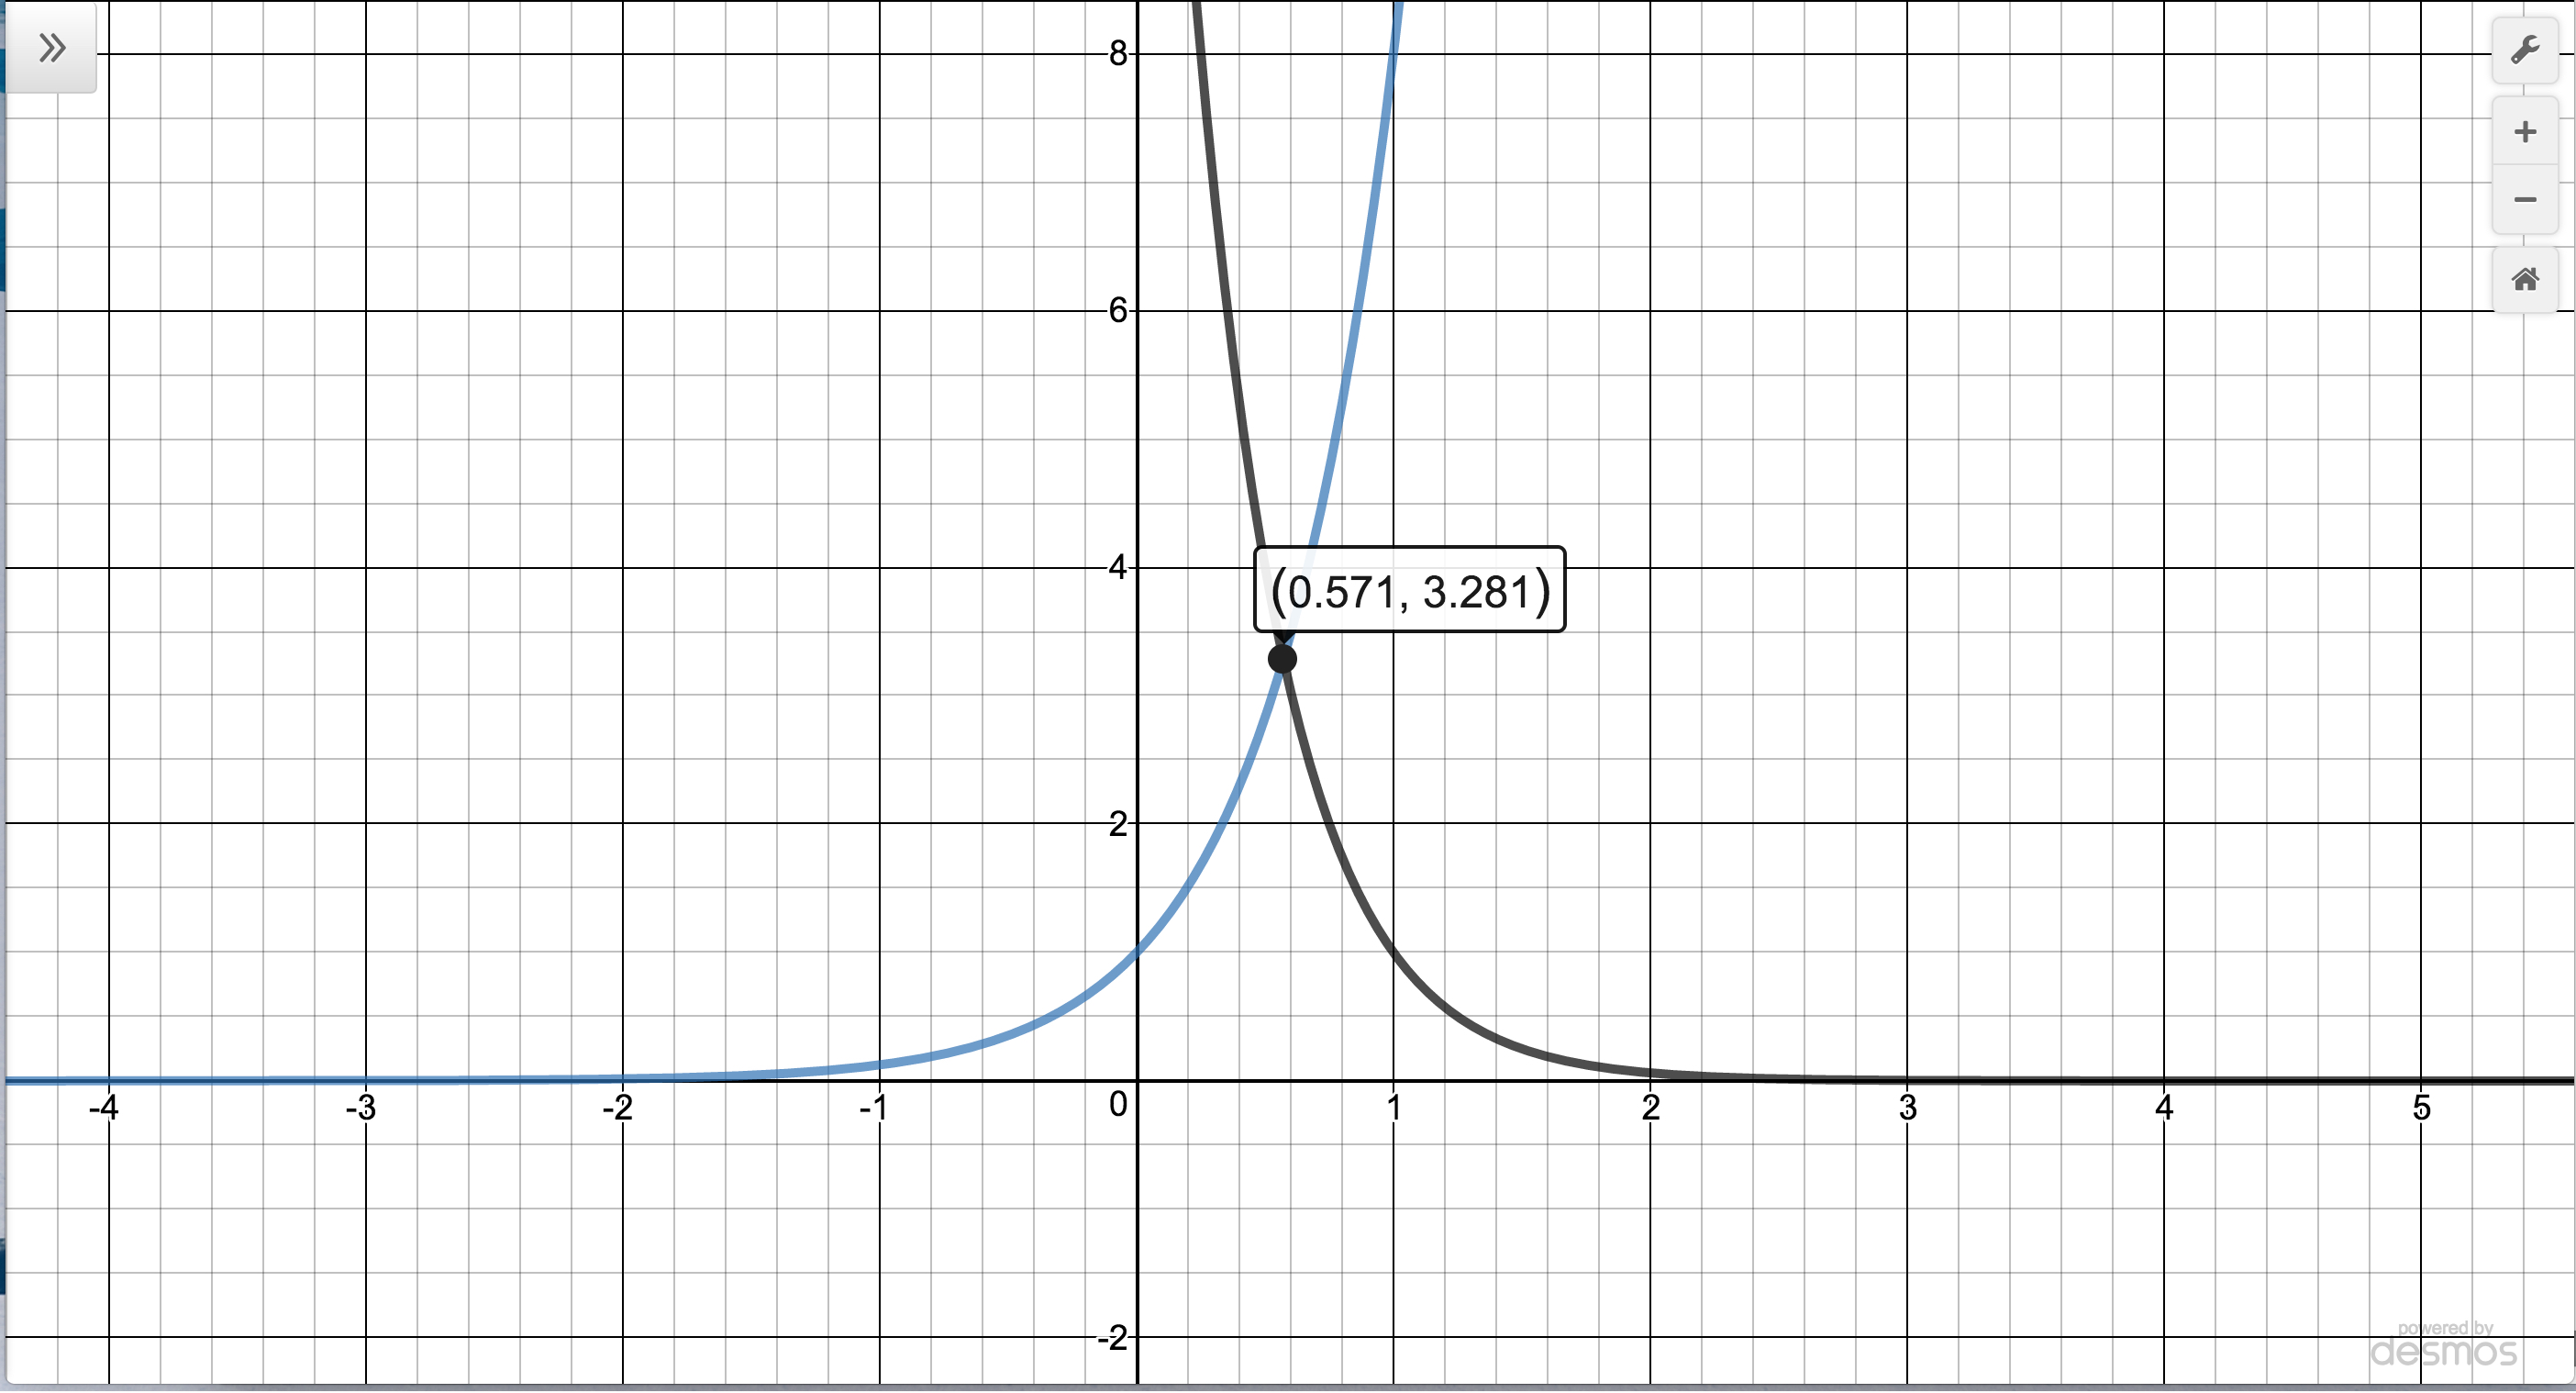
\includegraphics[width=3in]{./ExponentialEquationsandInequalitiesGraphics/ExpEqnEx01.jpg} &

 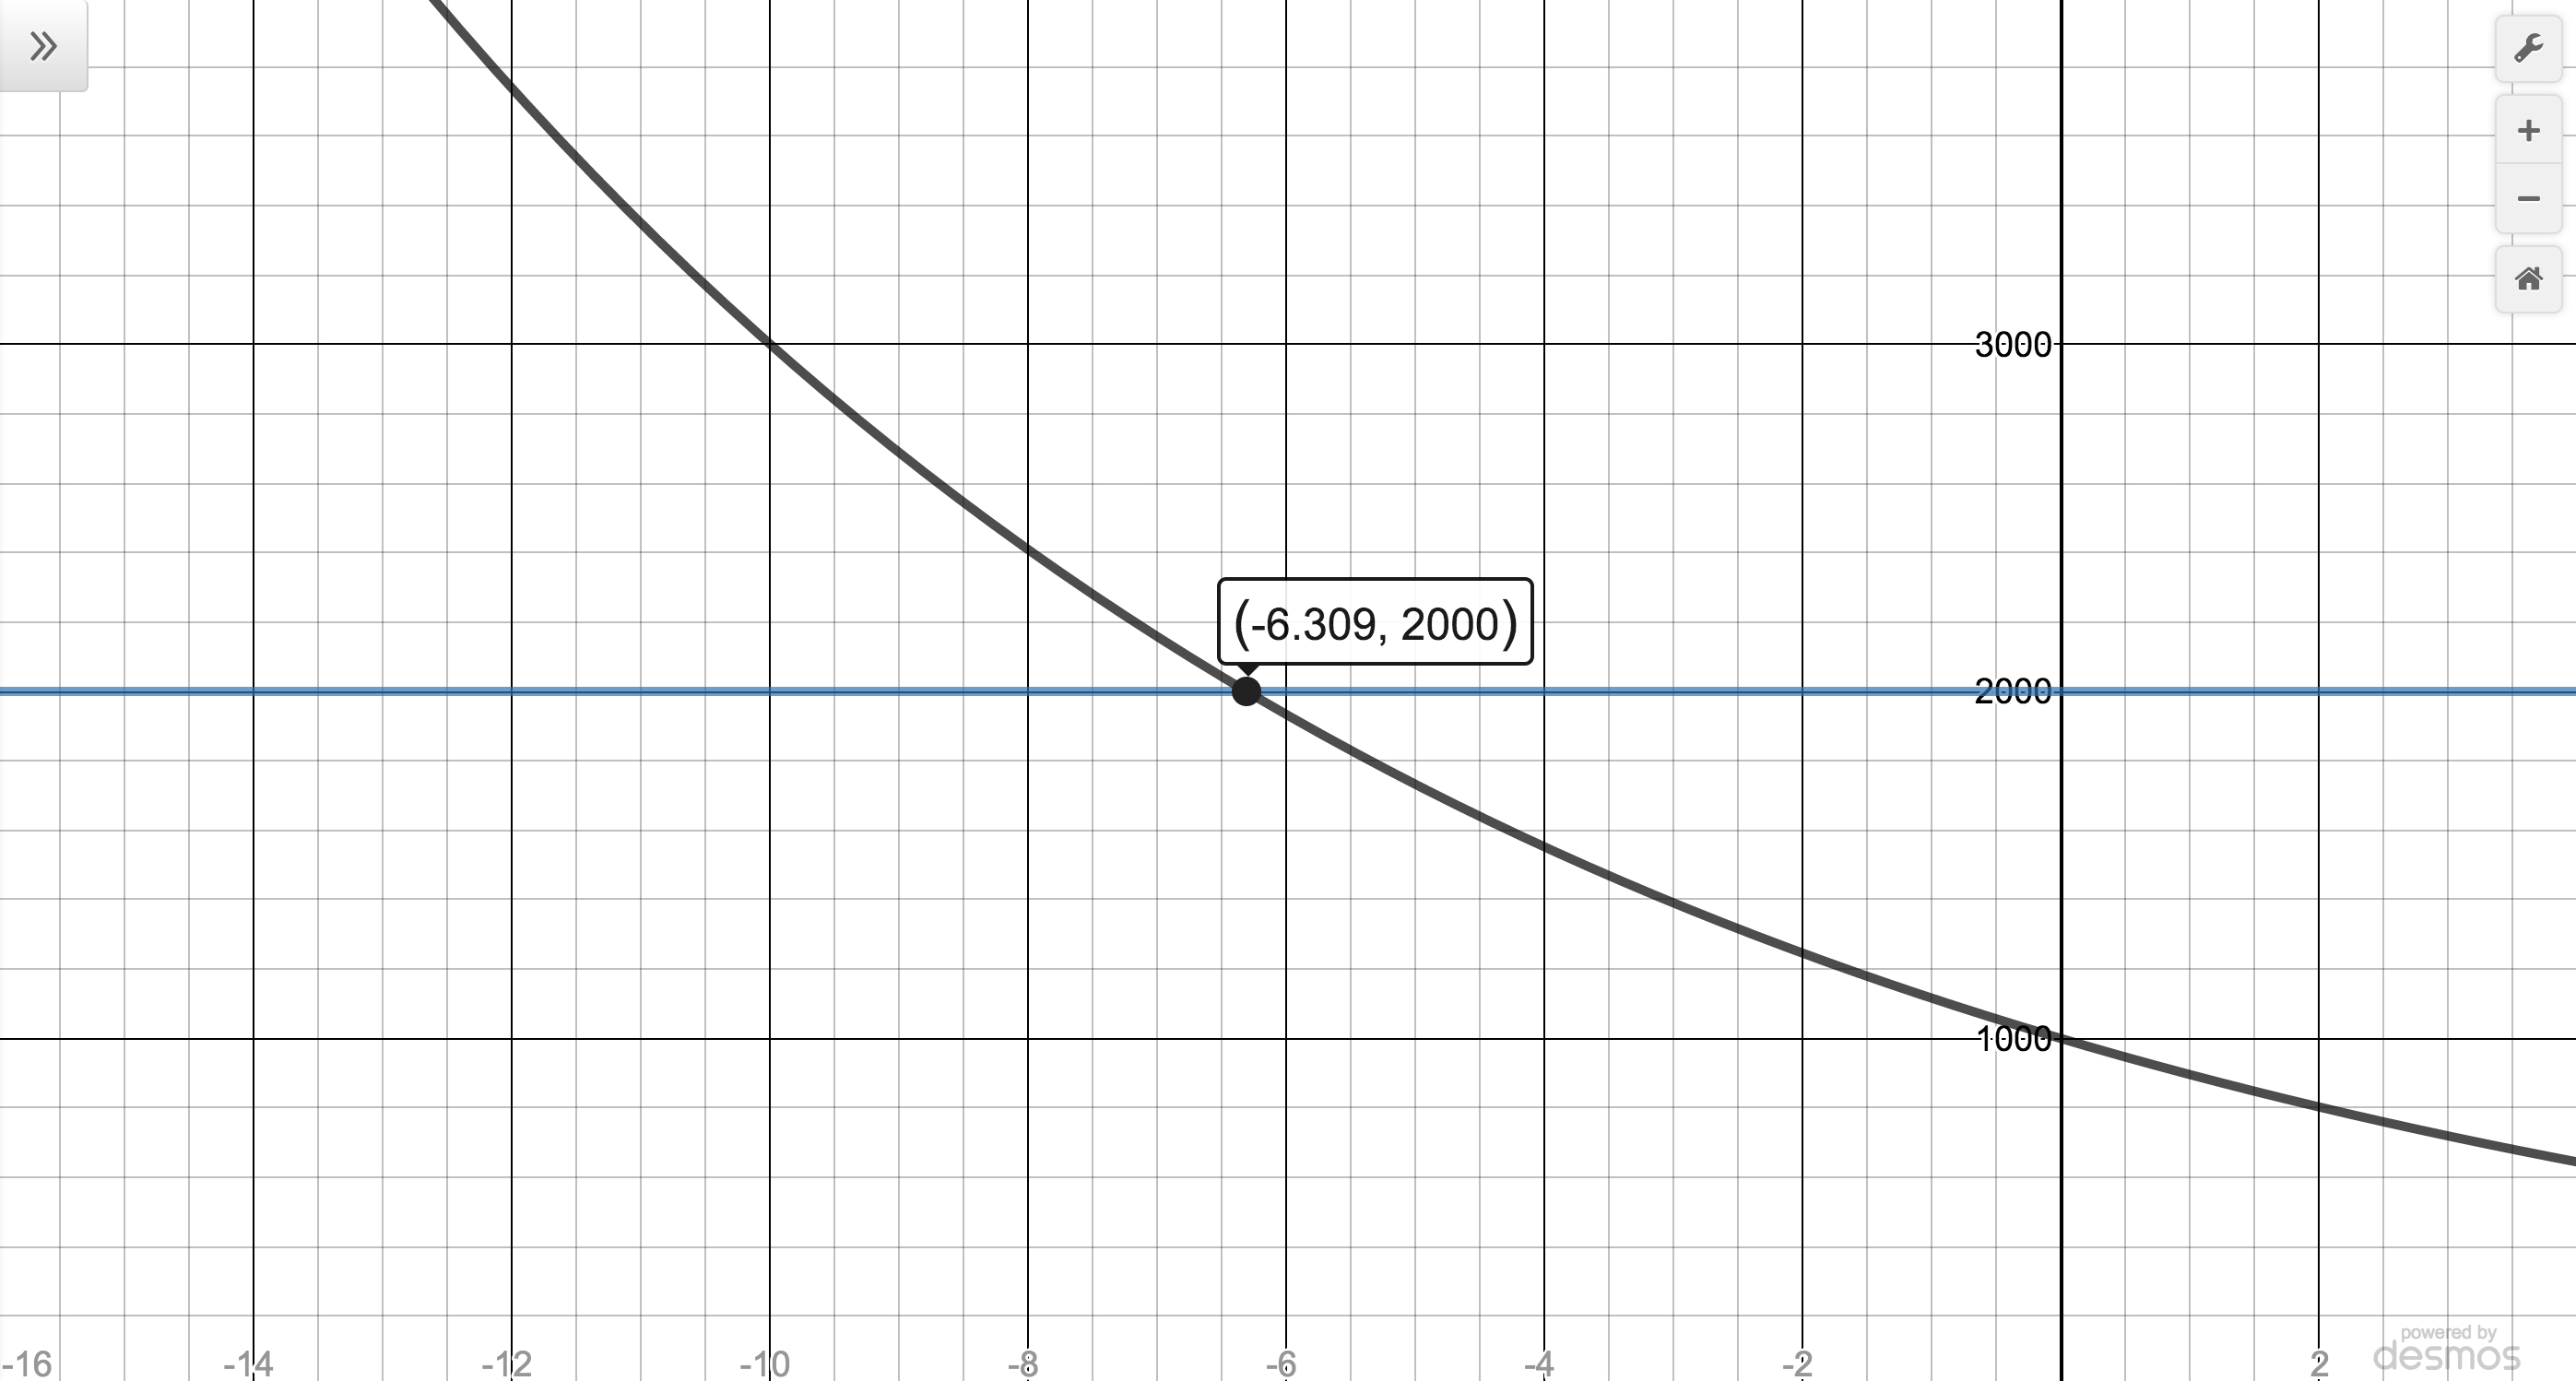
\includegraphics[width=3in]{./ExponentialEquationsandInequalitiesGraphics/ExpEqnEx02.jpg} \\

Checking $2^{3x} = 16^{1-x}$ 
 
 &
 
 Checking $2000 = 1000 \cdot 3^{-0.1 t}$
 
\end{tabular}

\end{center}

\item  We first note that we can rewrite the equation $9 \cdot 3^{x} = 7^{2x}$ as $3^2 \cdot 3^x = 7^{2x}$ to obtain $3^{x+2} = 7^{2x}$. 

\smallskip

Since it is not convenient to express both sides as a power of $3$ (or $7$ for that matter) we use the natural log:  $\ln\left(3^{x+2}\right) = \ln\left(7^{2x}\right)$.  

\smallskip

The power rule gives $(x+2) \ln(3) = 2x \ln(7)$.  Even though this equation appears very complicated, keep in mind that $\ln(3)$ and $\ln(7)$ are just constants.  

\smallskip

The equation $(x+2) \ln(3) = 2x \ln(7)$ is actually a linear equation (do you see why?) and as such we gather all of the terms with $x$ on one side, and the constants on the other.  We then divide both sides by the coefficient of $x$, which we obtain by factoring.

\[ \begin{array}{rclr}
(x+2) \ln(3) & = & 2x \ln(7) & \\

x \ln(3) + 2 \ln(3) & = & 2x \ln(7) & \\
2 \ln(3) & = & 2x \ln(7) - x \ln(3) & \\
2 \ln(3) & = & x (2 \ln(7) - \ln(3)) & \mbox{Factor.}\\
x & = & \frac{2 \ln(3)}{2\ln(7) - \ln(3)} & \\ [4pt]
\end{array}\]

We see the graphs of $f(x) = 9 \cdot 3^{x}$ and $g(x) = 7^{2x}$ intersect at $x  \approx 0.787 \approx  \frac{2 \ln(3)}{2\ln(7) - \ln(3)}$.

\item  Our objective in solving  $75 = \frac{100}{1 + 3e^{-2t}}$ is to first isolate the exponential.  

\smallskip

To that end, we clear denominators and get $75\left(1 + 3e^{-2t}\right) = 100$, or $75 + 225e^{-2t} =100$.   We get  $225e^{-2t} = 25$, so finally, $e^{-2t} = \frac{1}{9}$.    

\smallskip

Taking the natural log of both sides gives $\ln\left(e^{-2t}\right) = \ln\left( \frac{1}{9} \right)$.  Since natural log is log base $e$, $\ln\left(e^{-2t}\right) = -2t$.  Likewise, we use the Power Rule to rewrite $\ln\left( \frac{1}{9} \right) = -\ln(9)$.  

\smallskip

Putting these two steps together, we simplify $\ln\left(e^{-2t}\right) = \ln\left( \frac{1}{9} \right)$ to   $-2t = -\ln(9)$.  We arrive at our solution, $t = \frac{\ln(9)}{2}$ which simplifies to $t = \ln(3)$. (Can you explain why?)  

\smallskip

 To check, we see the graphs of  $f(x) = 75$ and $g(x) = \frac{100}{1 + 3e^{-2x}}$,  intersect at $x \approx 1.099 \approx \ln(3)$.

\begin{center}

\begin{tabular}{cc}

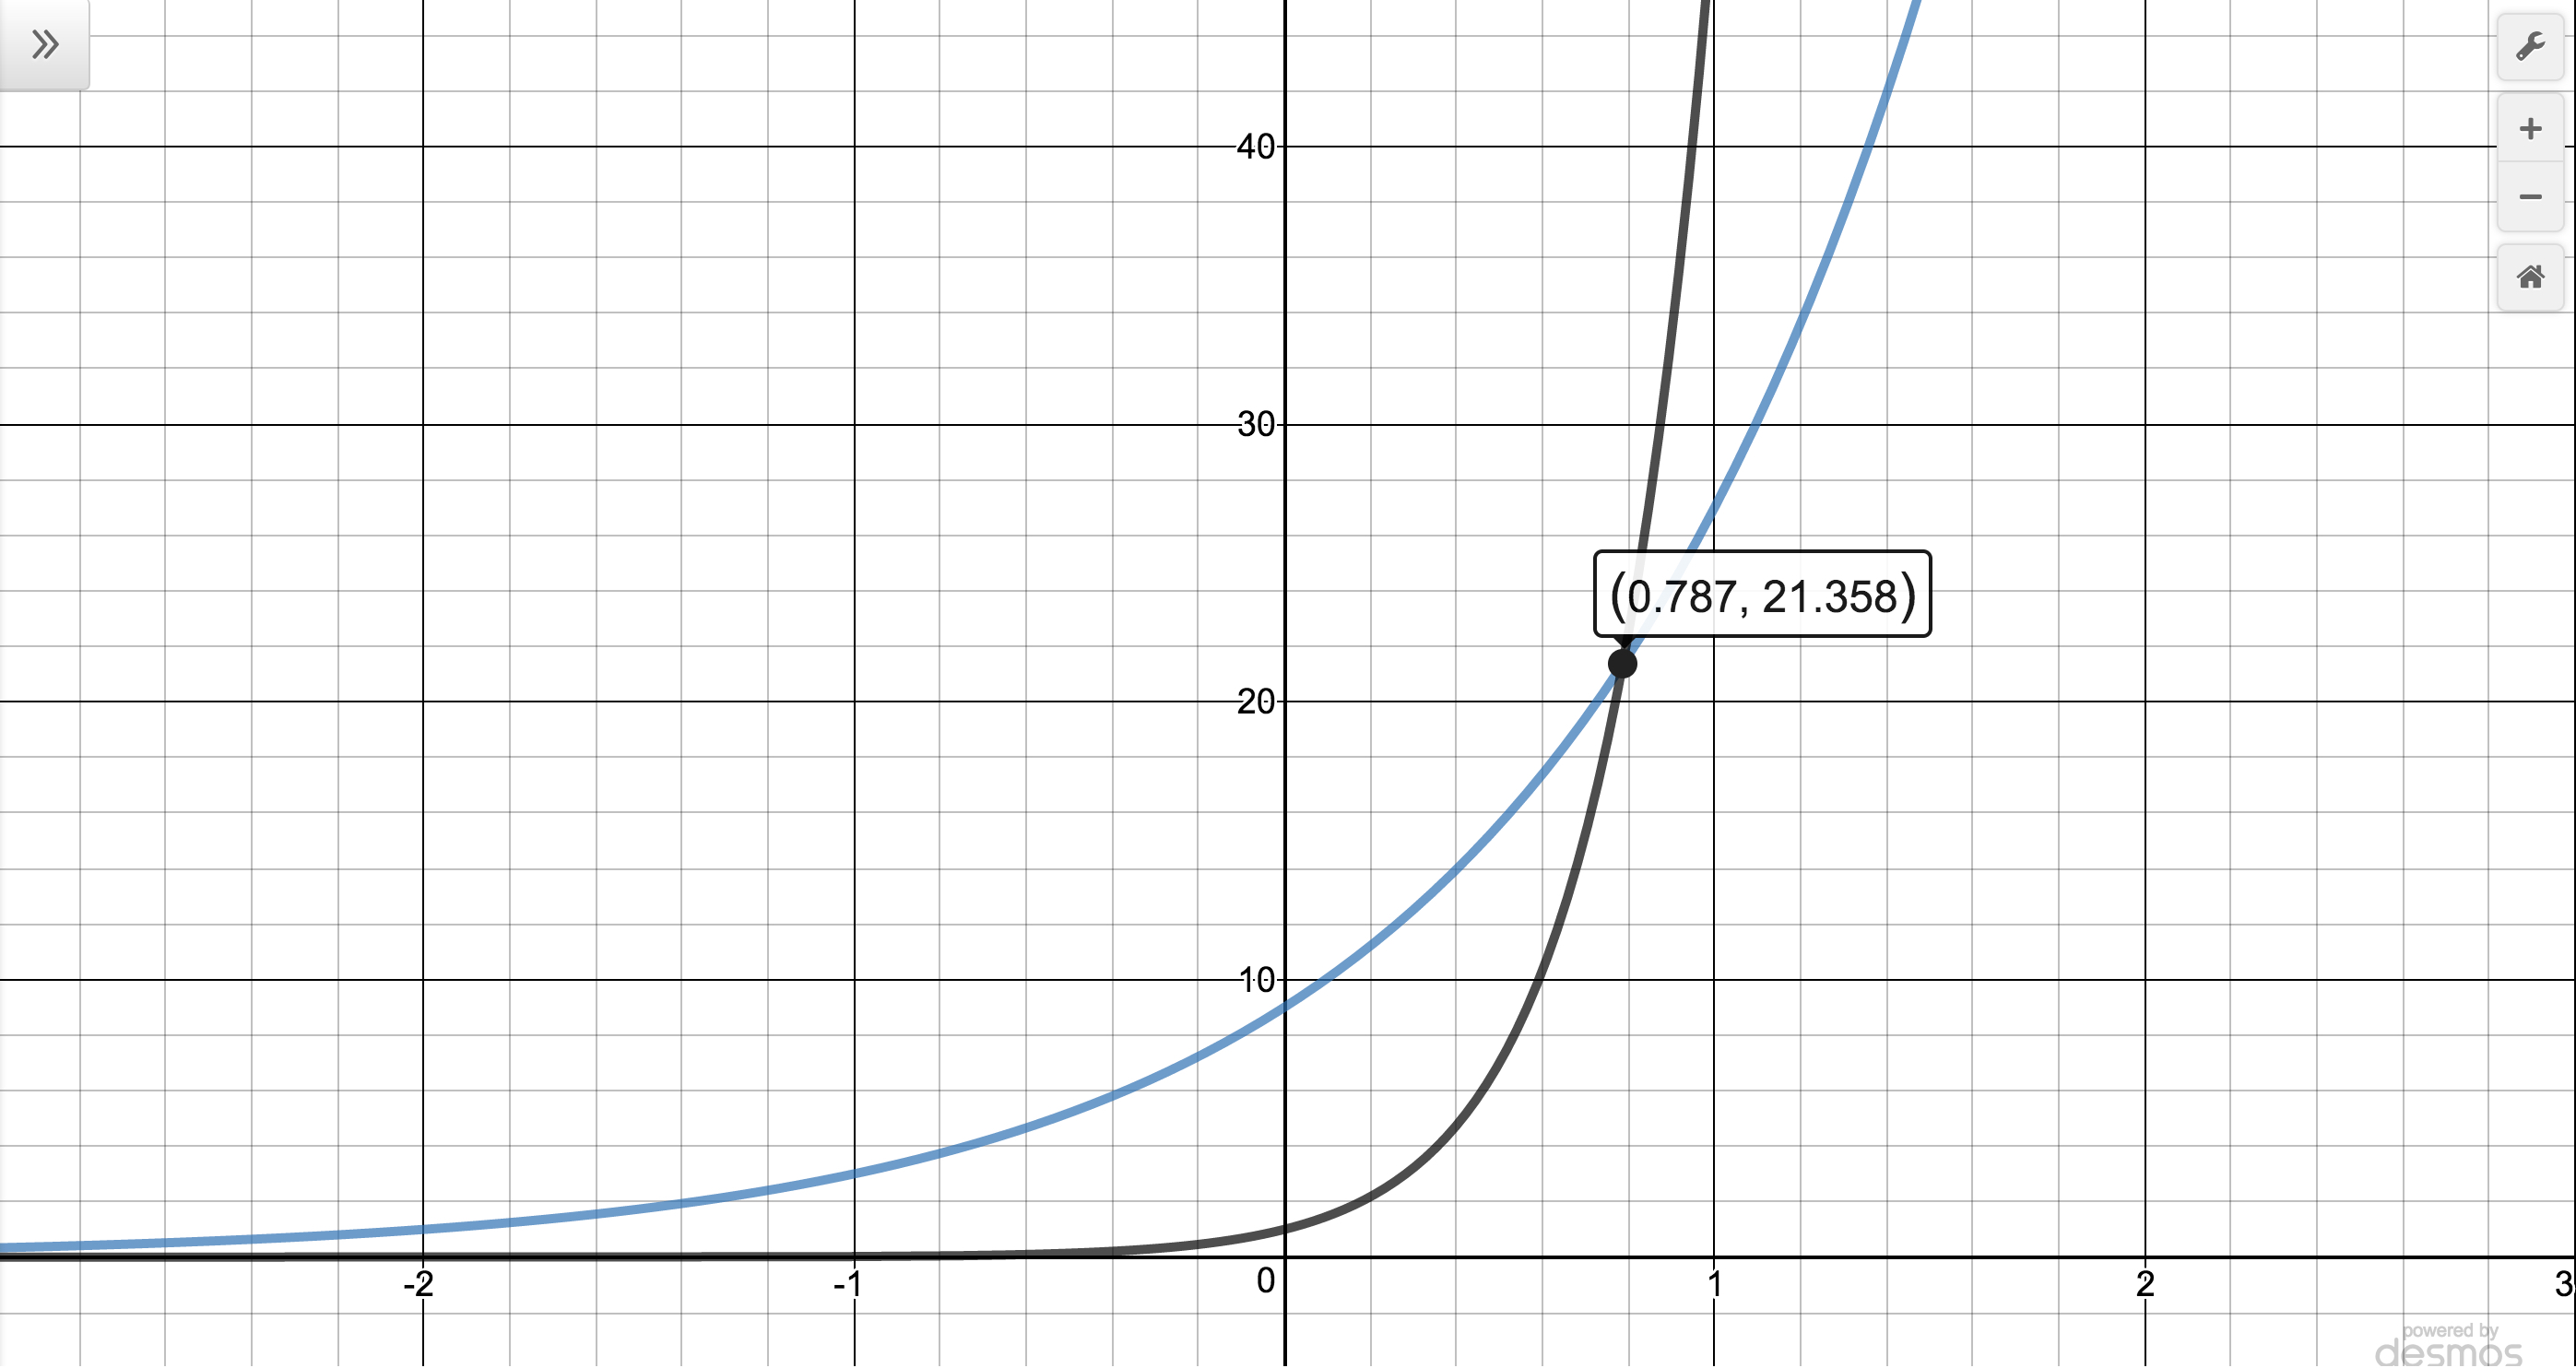
\includegraphics[width=3in]{./ExponentialEquationsandInequalitiesGraphics/ExpEqnEx03.jpg} &

 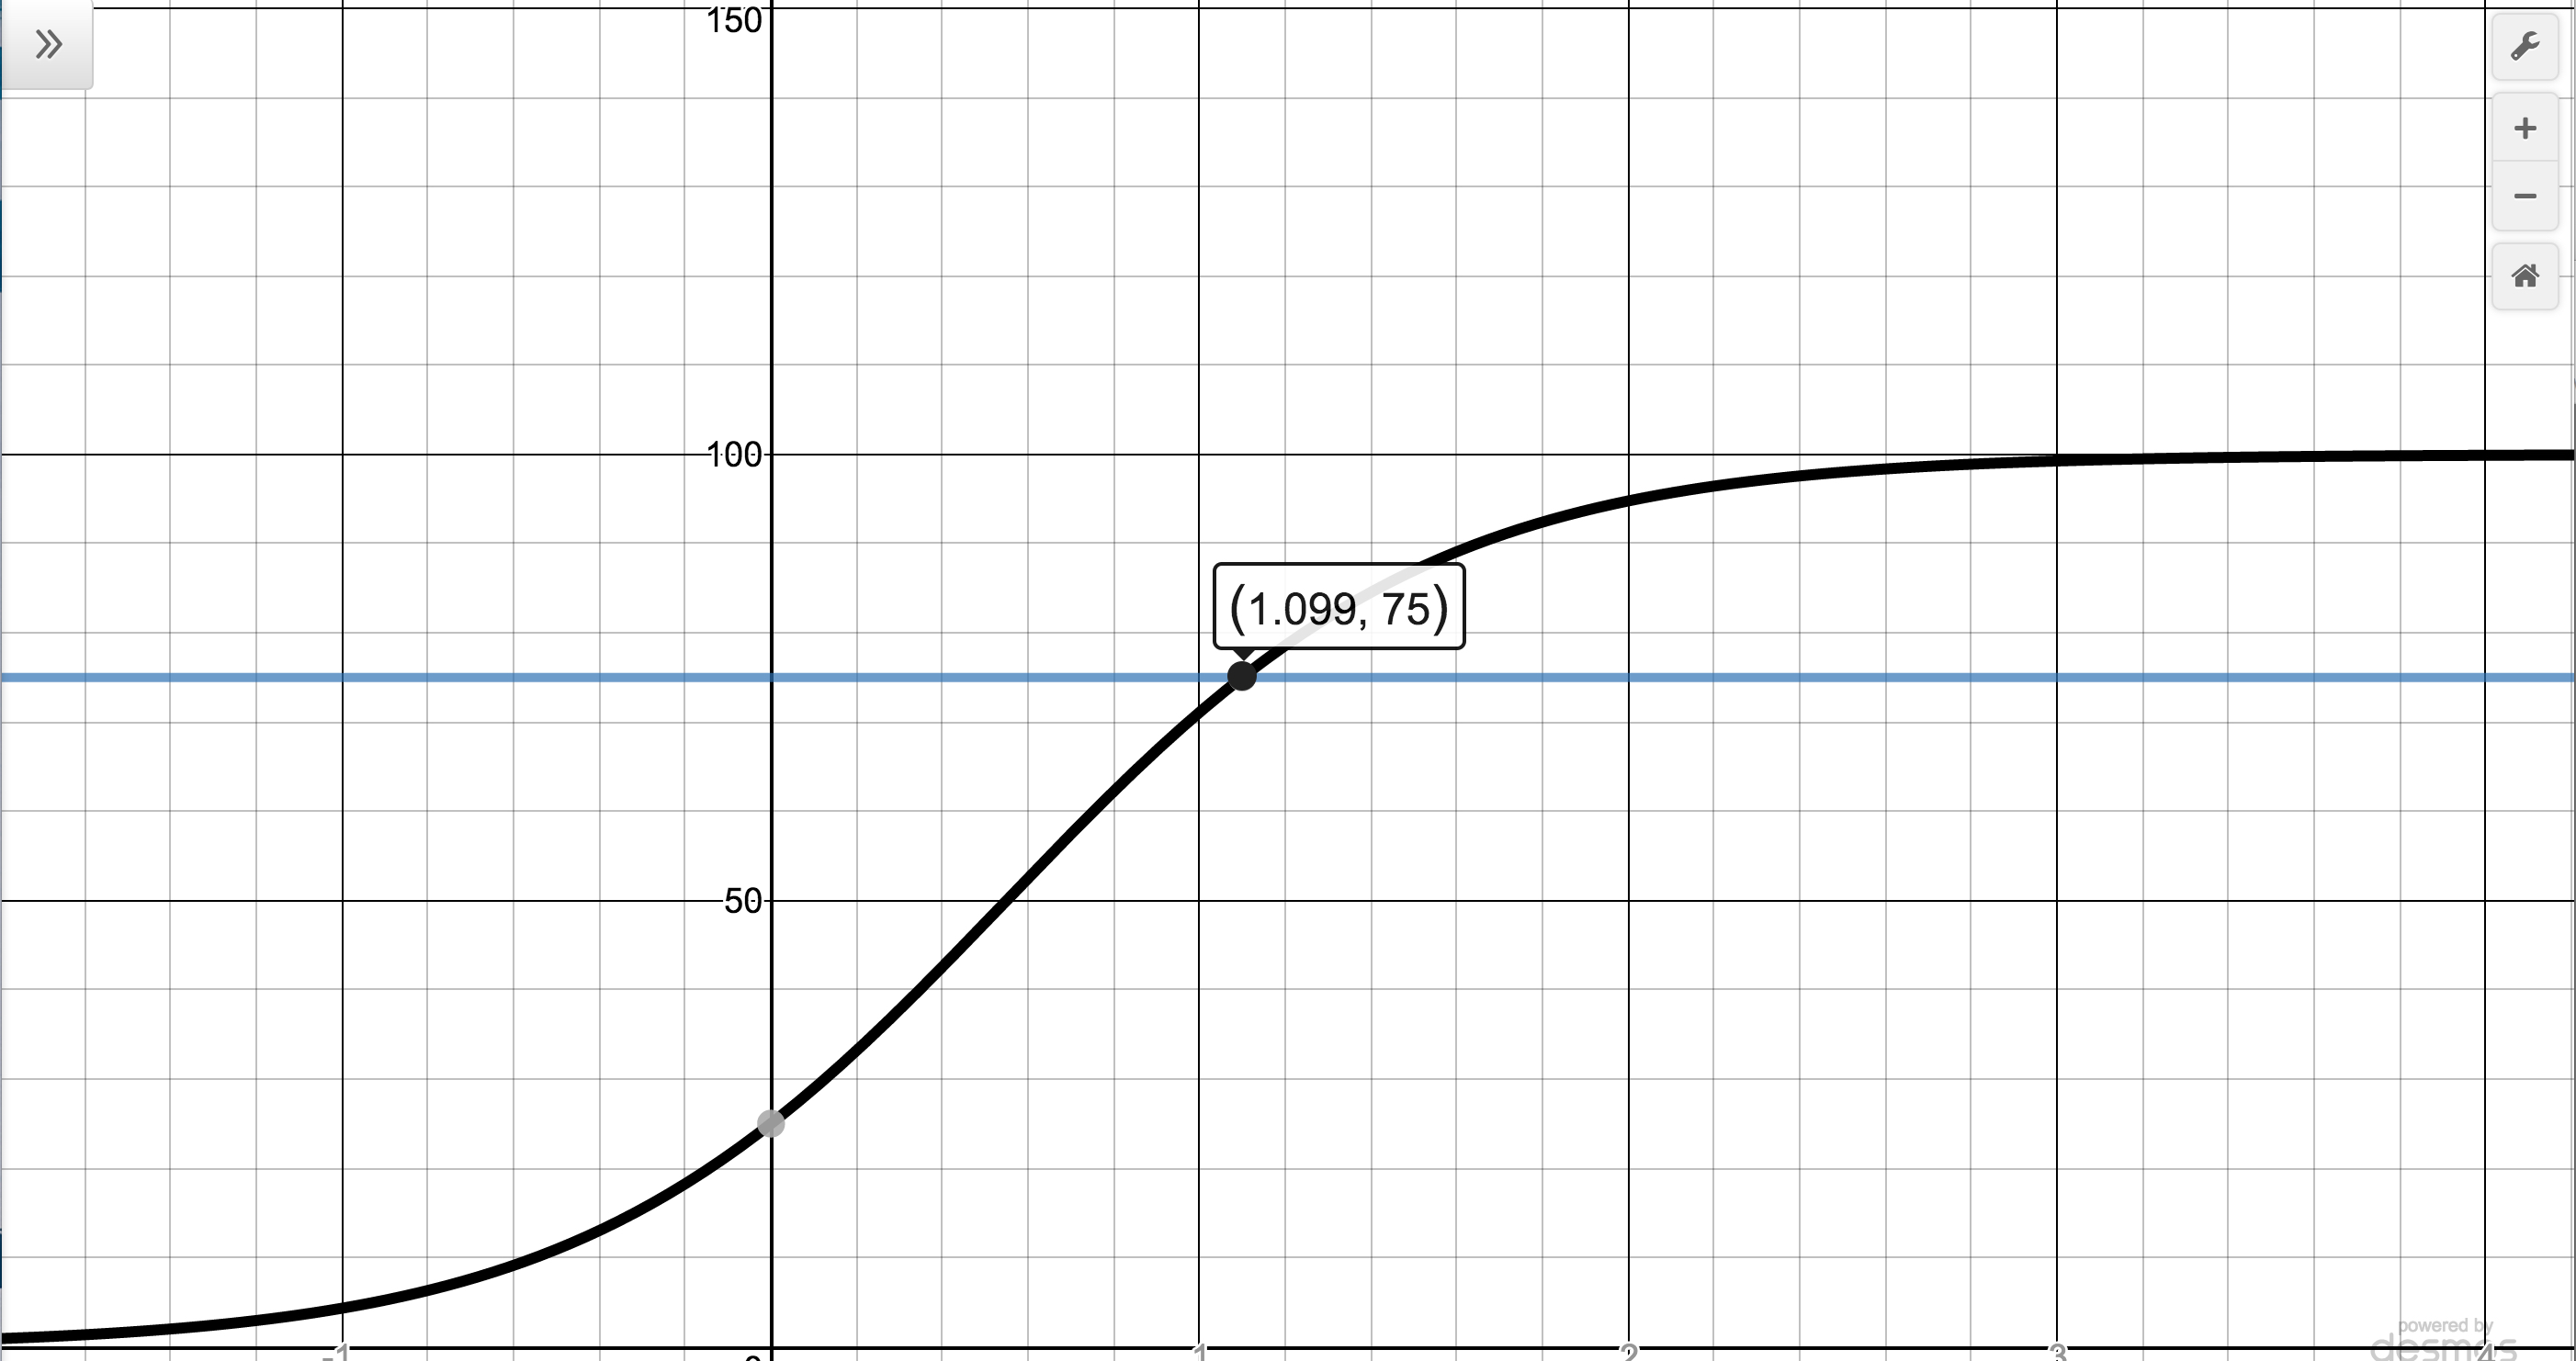
\includegraphics[width=3in]{./ExponentialEquationsandInequalitiesGraphics/ExpEqnEx04.jpg} \\

Checking $9 \cdot 3^{x} = 7^{2x}$ 
 
 &
 
 Checking $75 = \frac{100}{1 + 3e^{-2t}}$
 
\end{tabular}

\end{center}

\item  We start solving $25^{x} = 5^{x} + 6$ by rewriting $25 = 5^2$ so that we have $\left(5^2\right)^{x} = 5^{x} + 6$, or $5^{2x} = 5^{x} + 6$.  

\smallskip

Even though we have a common base, having two terms on the right hand side of the equation foils our plan of equating exponents or taking logs.  

\smallskip

If we stare at this long enough, we notice that we have three terms with the exponent on one term exactly twice that of another. To our surprise and delight, we have a  `quadratic in disguise'.  

Letting $u = 5^{x}$,  we have $u^2 = \left(5^{x}\right)^2 = 5^{2x}$ so the equation $5^{2x} = 5^{x} + 6$ becomes $u^2 = u + 6$.  Solving this as $u^2 - u - 6=0$ gives $u = -2$ or $u = 3$.  Since $u = 5^{x}$, we have $5^{x} = -2$ or $5^{x} = 3$.  

\smallskip

Since $5^{x} = -2$ has no real solution,\footnote{Why not?} we focus on $5^{x} = 3$.  Since it isn't convenient to express $3$ as a power of $5$, we take natural logs and get $\ln\left(5^{x}\right) = \ln(3)$ so that $x \ln(5) = \ln(3)$ or $x = \frac{\ln(3)}{\ln(5)}$.  

\smallskip

We see the graphs of $f(x) = 25^{x}$ and $g(x) = 5^{x} + 6$ intersect at $x \approx 0.683 \approx \frac{\ln(3)}{\ln(5)} $.

\item  Clearing the denominator in  $\frac{e^{x} - e^{-x}}{2} = 5$ gives $e^{x} - e^{-x} = 10$, at which point we pause to consider how to proceed. Rewriting $e^{-x} = \frac{1}{e^{x}}$, we see we have another denominator to clear:  $e^{x} - \frac{1}{e^{x}} = 10$. 

\smallskip

Doing so gives $e^{2x} - 1 = 10e^{x}$, which, once again fits the criteria of being a `quadratic in disguise.' 

\smallskip

If we let $u = e^{x}$, then $u^2 = e^{2x}$ so the equation $e^{2x} - 1 = 10e^{x}$ can be viewed as $u^2-1 = 10u$.  Solving $u^2 - 10u - 1 = 0$ using the quadratic formula gives $u = 5 \pm \sqrt{26}$.  

\smallskip

From this, we have $e^{x} = 5 \pm \sqrt{26}$.  Since $5 - \sqrt{26} < 0$, we get no real solution to $e^{x} = 5 - \sqrt{26}$ (why not?) but for $e^{x} = 5 + \sqrt{26}$, we take natural logs to obtain $x = \ln\left(5 + \sqrt{26}\right)$.  

\smallskip

We see the graphs of  $f(x) = \frac{e^{x} - e^{-x}}{2}$ and $g(x) = 5$ intersect at $x \approx 2.312 \approx \ln\left(5 + \sqrt{26}\right)$.

\begin{center}

\begin{tabular}{cc}

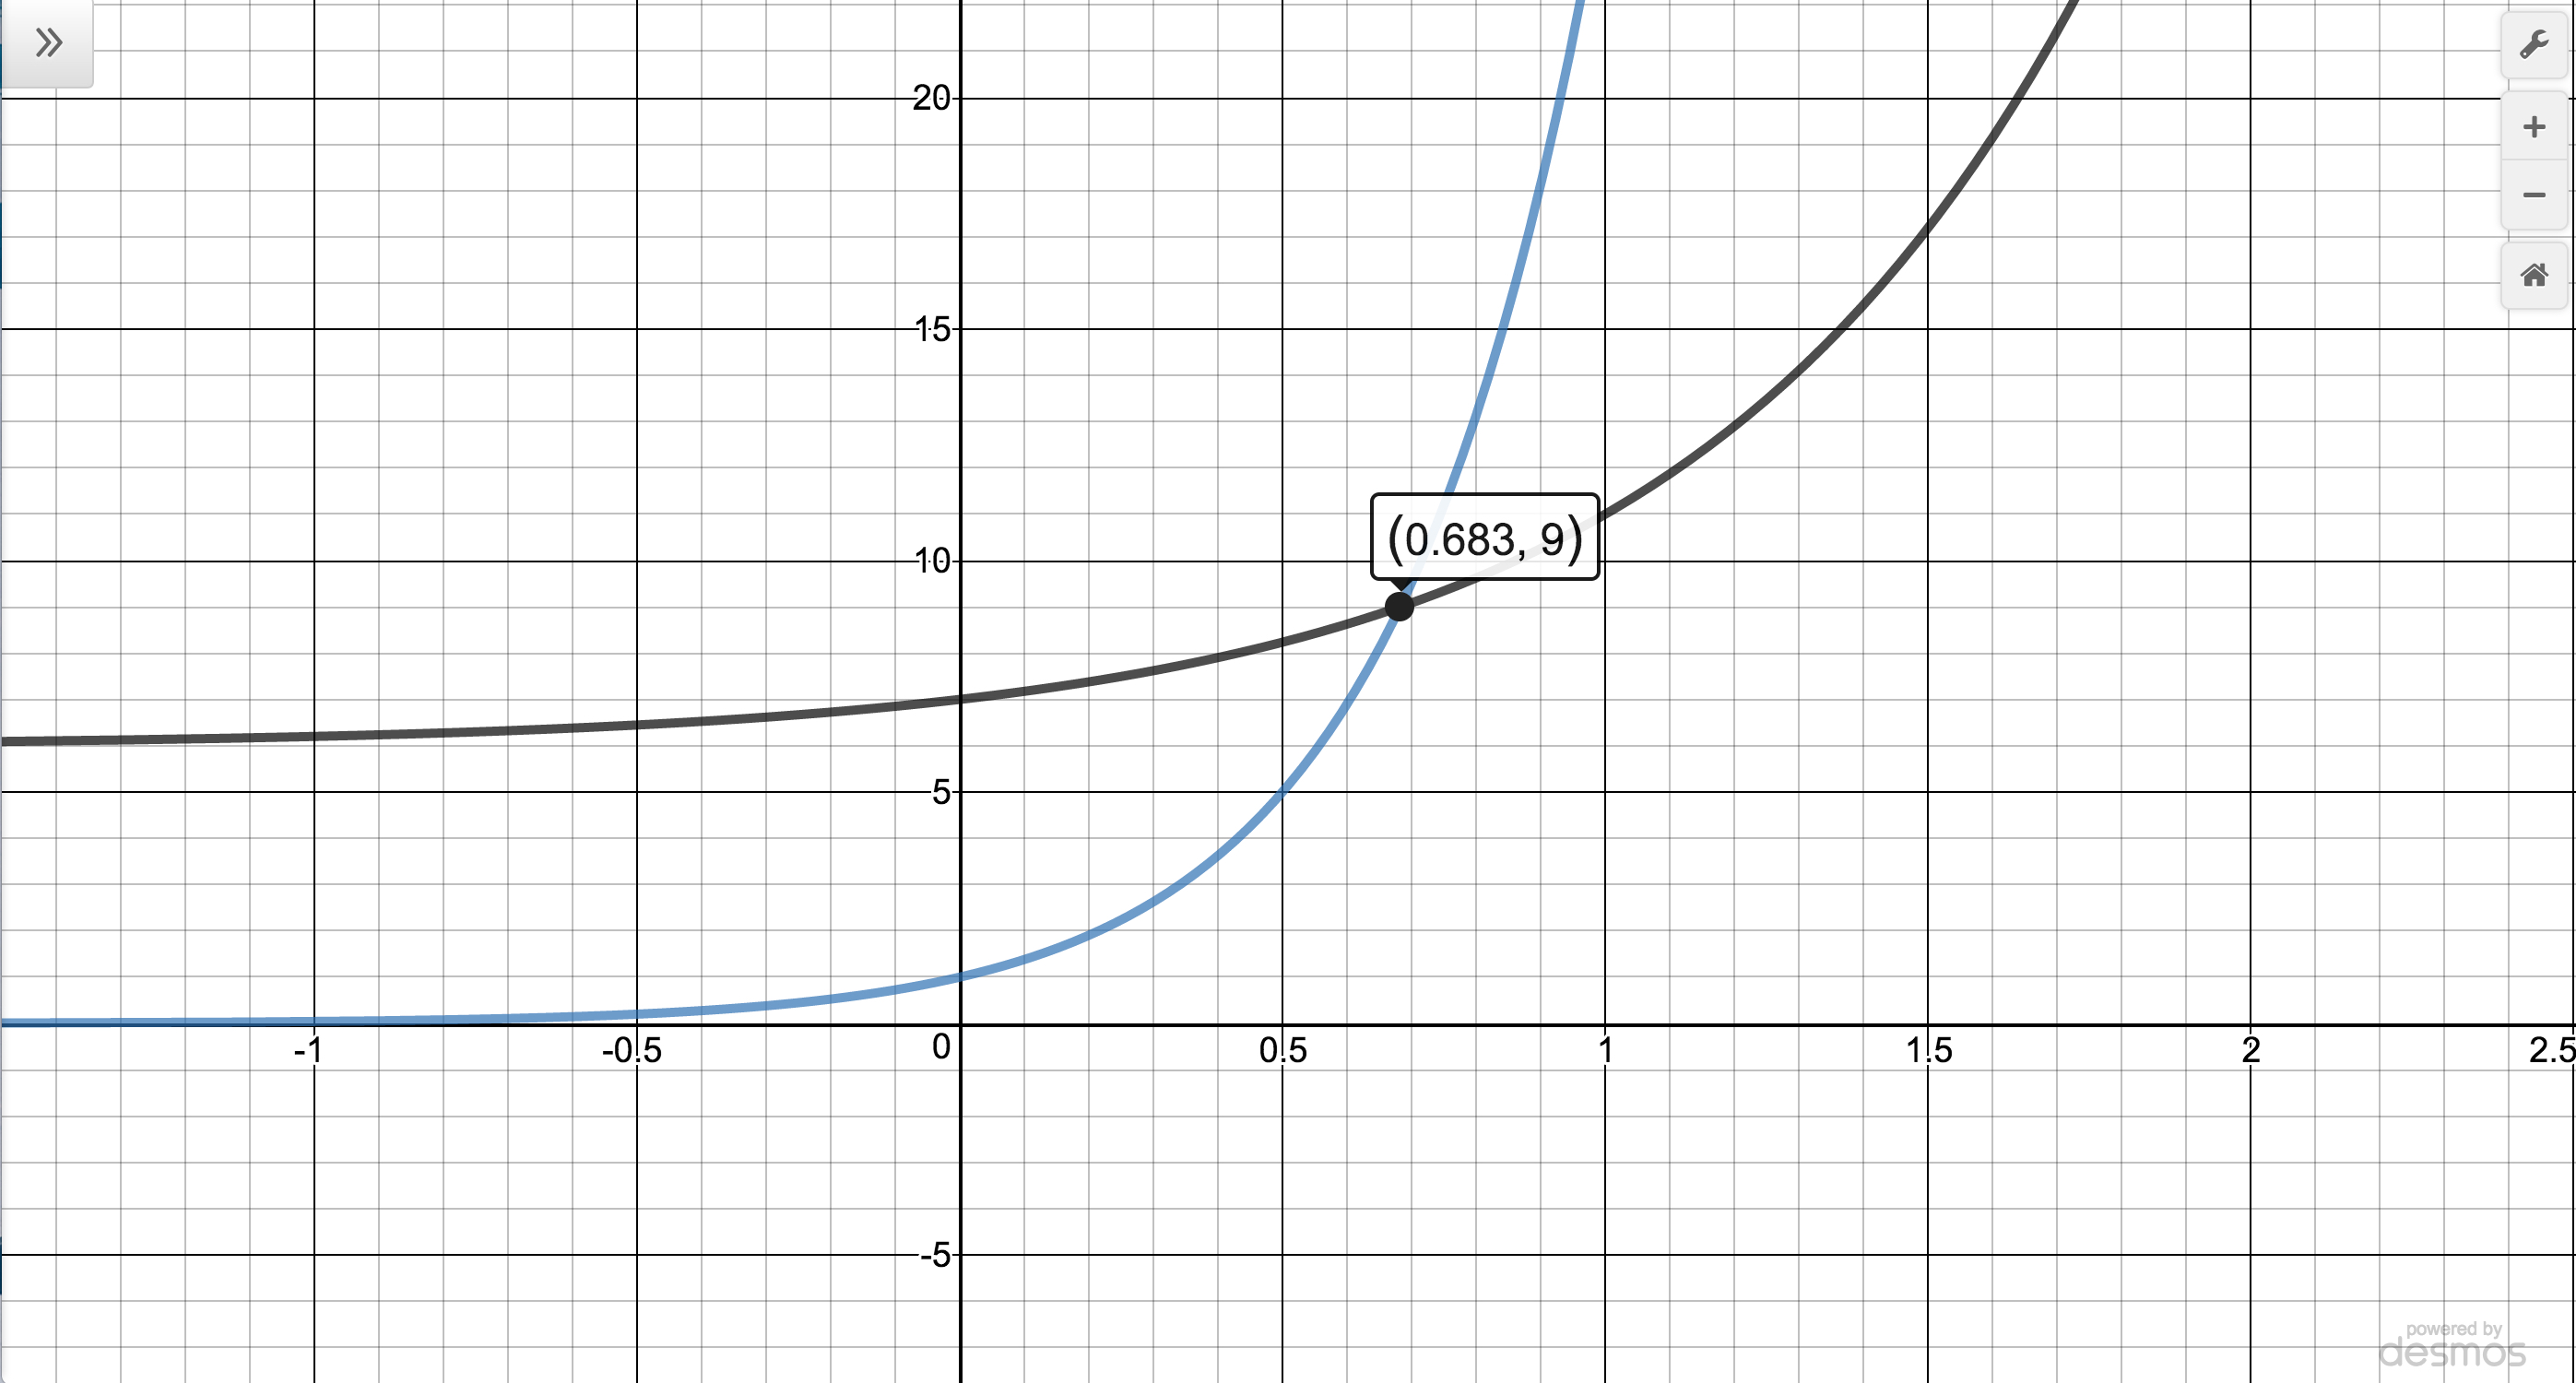
\includegraphics[width=3in]{./ExponentialEquationsandInequalitiesGraphics/ExpEqnEx05.jpg} &

 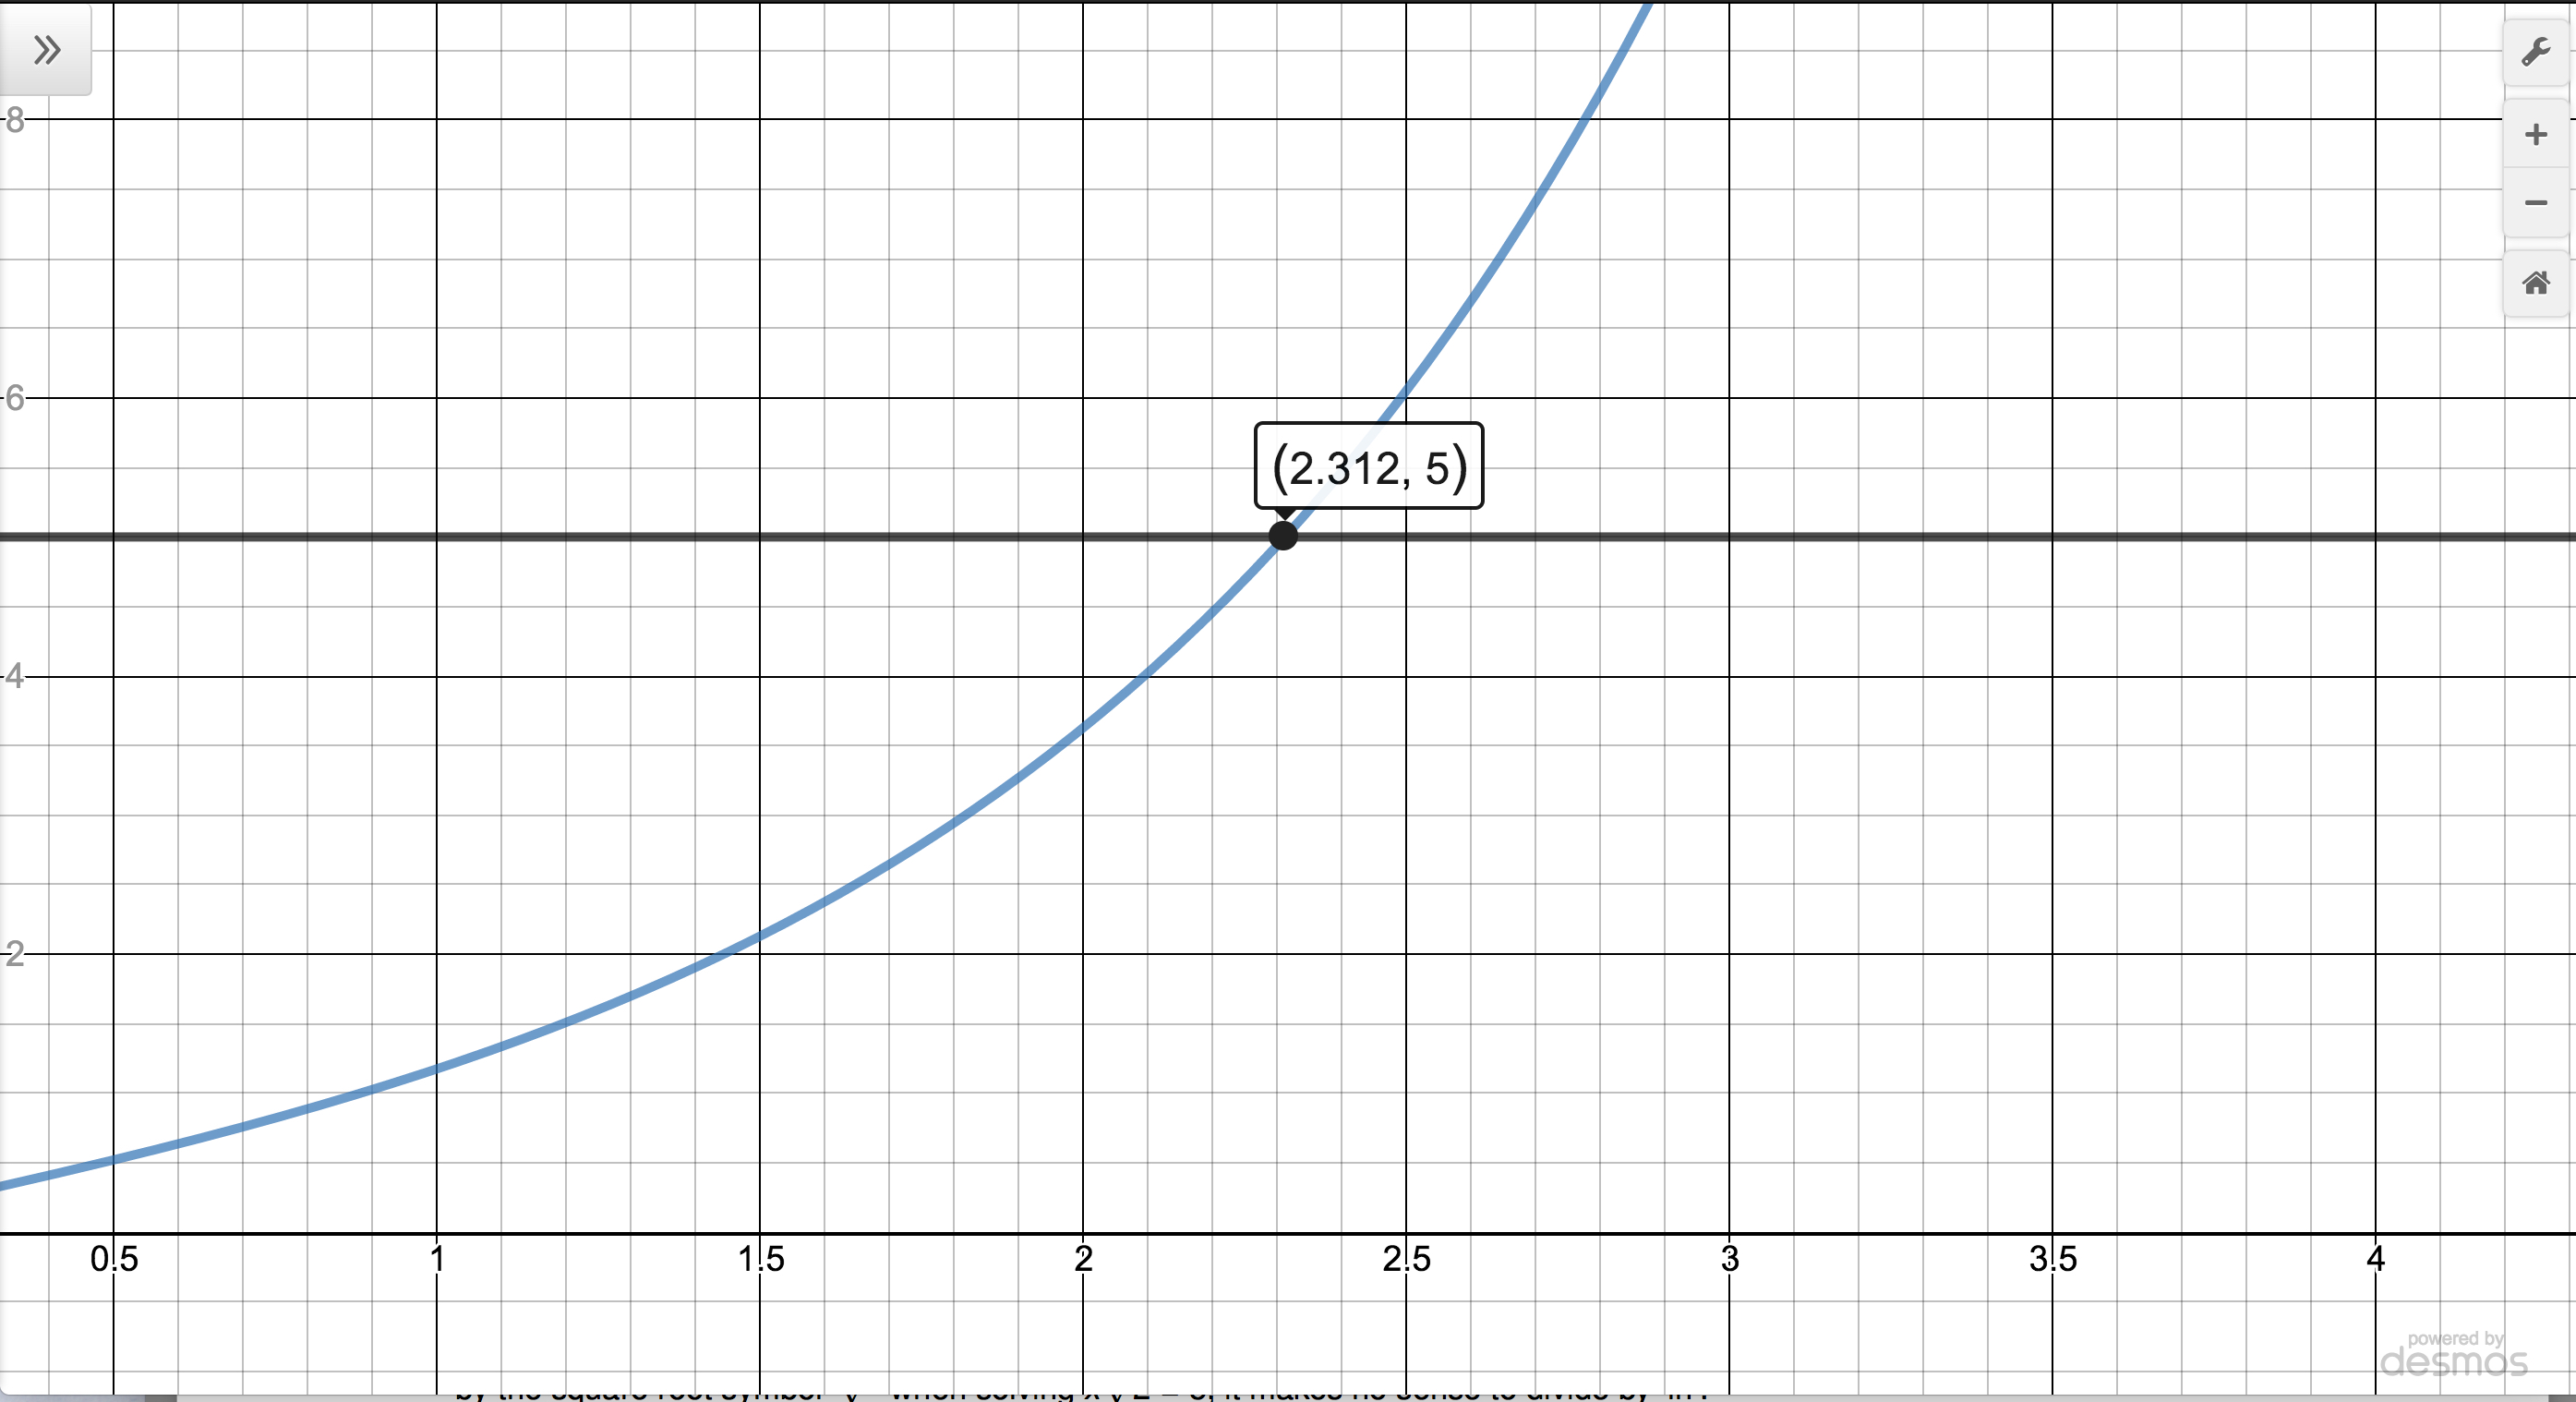
\includegraphics[width=3in]{./ExponentialEquationsandInequalitiesGraphics/ExpEqnEx06.jpg} \\

 Checking $25^{x} = 5^{x} + 6$
 
 &
 
 Checking   $\frac{e^{x} - e^{-x}}{2} = 5$
 
\end{tabular}

\end{center}


\end{enumerate}

\qed

\end{ex}

Note that verifying our solutions to the equations in Example \ref{expeqnsex1} \textit{analytically} holds great educational value, since it reviews many of the properties of logarithms and exponents in tandem.

\smallskip

For example, to verify our solution to  $2000 = 1000 \cdot 3^{-0.1 t}$, we substitute $t = -\frac{10\ln(2)}{\ln(3)}$ and check: 
\[ \begin{array}{rclr}

2000 & \stackrel{?}{=} & 1000 \cdot 3^{-0.1 \left(-\frac{10\ln(2)}{\ln(3)}\right)} & \\
2000 & \stackrel{?}{=} & 1000 \cdot 3^{\frac{\ln(2)}{\ln(3)}} & \\
2000 & \stackrel{?}{=} & 1000 \cdot 3^{\log_{3}(2)} & \mbox{Change of Base}\\
2000 & \stackrel{?}{=} & 1000 \cdot 2 & \mbox{Inverse Property}\\
2000 & \stackrel{\checkmark}{=} & 2000 & \\

\end{array}\]

We strongly encourage the reader to check the remaining equations analytically as well.

\smallskip

Since exponential functions are continuous on their domains, the Intermediate Value Theorem \ref{IVT} applies. This allows us to solve inequalities using sign diagrams as demonstrated below.

\begin{ex}  Solve the following inequalities.  Check your answer graphically.
\label{expineq}

\begin{multicols}{3}

\begin{enumerate}

\item \label{canuselogsex} $2^{x^2-3x} - 16 \geq 0$

\item  $\dfrac{e^{x}}{e^{x}-4} \leq 3$

\item  $t e^{2t} < 4t$

\end{enumerate}

\end{multicols}

\newpage

{\bf Solution.}

\begin{enumerate}

\item  Since we already have $0$ on one side of the inequality, we set $r(x) = 2^{x^2-3x} - 16$.  

\smallskip

The domain of $r$ is all real numbers, so to construct our sign diagram, we need to find the zeros of $r$.  

\smallskip

Setting $r(x) = 0$ gives $2^{x^2-3x} - 16 = 0$ or $2^{x^2-3x} = 16$.  Since $16 = 2^{4}$ we have $2^{x^2-3x} = 2^{4}$.   By the one-to-one property of exponential functions, $x^2 -3x = 4$ which gives $x=4$ and $x=-1$.  

\smallskip

From the sign diagram, we see $r(x) \geq 0$ on $(-\infty, -1] \cup [4, \infty)$, which is our solution.  

\smallskip

Graphing $r(x) = 2^{x^2-3x} - 16$,  we find it is on or above the line $y=0$ (the $x$-axis) precisely on the intervals  $(-\infty, -1]$ and $ [4, \infty)$ which checks our answer.

\begin{center}

\begin{tabular}{cc}

\begin{mfpic}[10]{-5}{5}{-1}{2}
\arrow \reverse \arrow \polyline{(-5,0),(5,0)}
\xmarks{-2,2}
\tlabel[cc](-3.5,1){$(+)$}
\tlabel[cc](-2,-1){$-1$}
\tlabel[cc](-2,1){$0$}
\tlabel[cc](0,1){$(-)$}
\tlabel[cc](2,-1){$4$}
\tlabel[cc](2,1){$0$}
\tlabel[cc](3.5,1){$(+)$}
\end{mfpic}

& 

 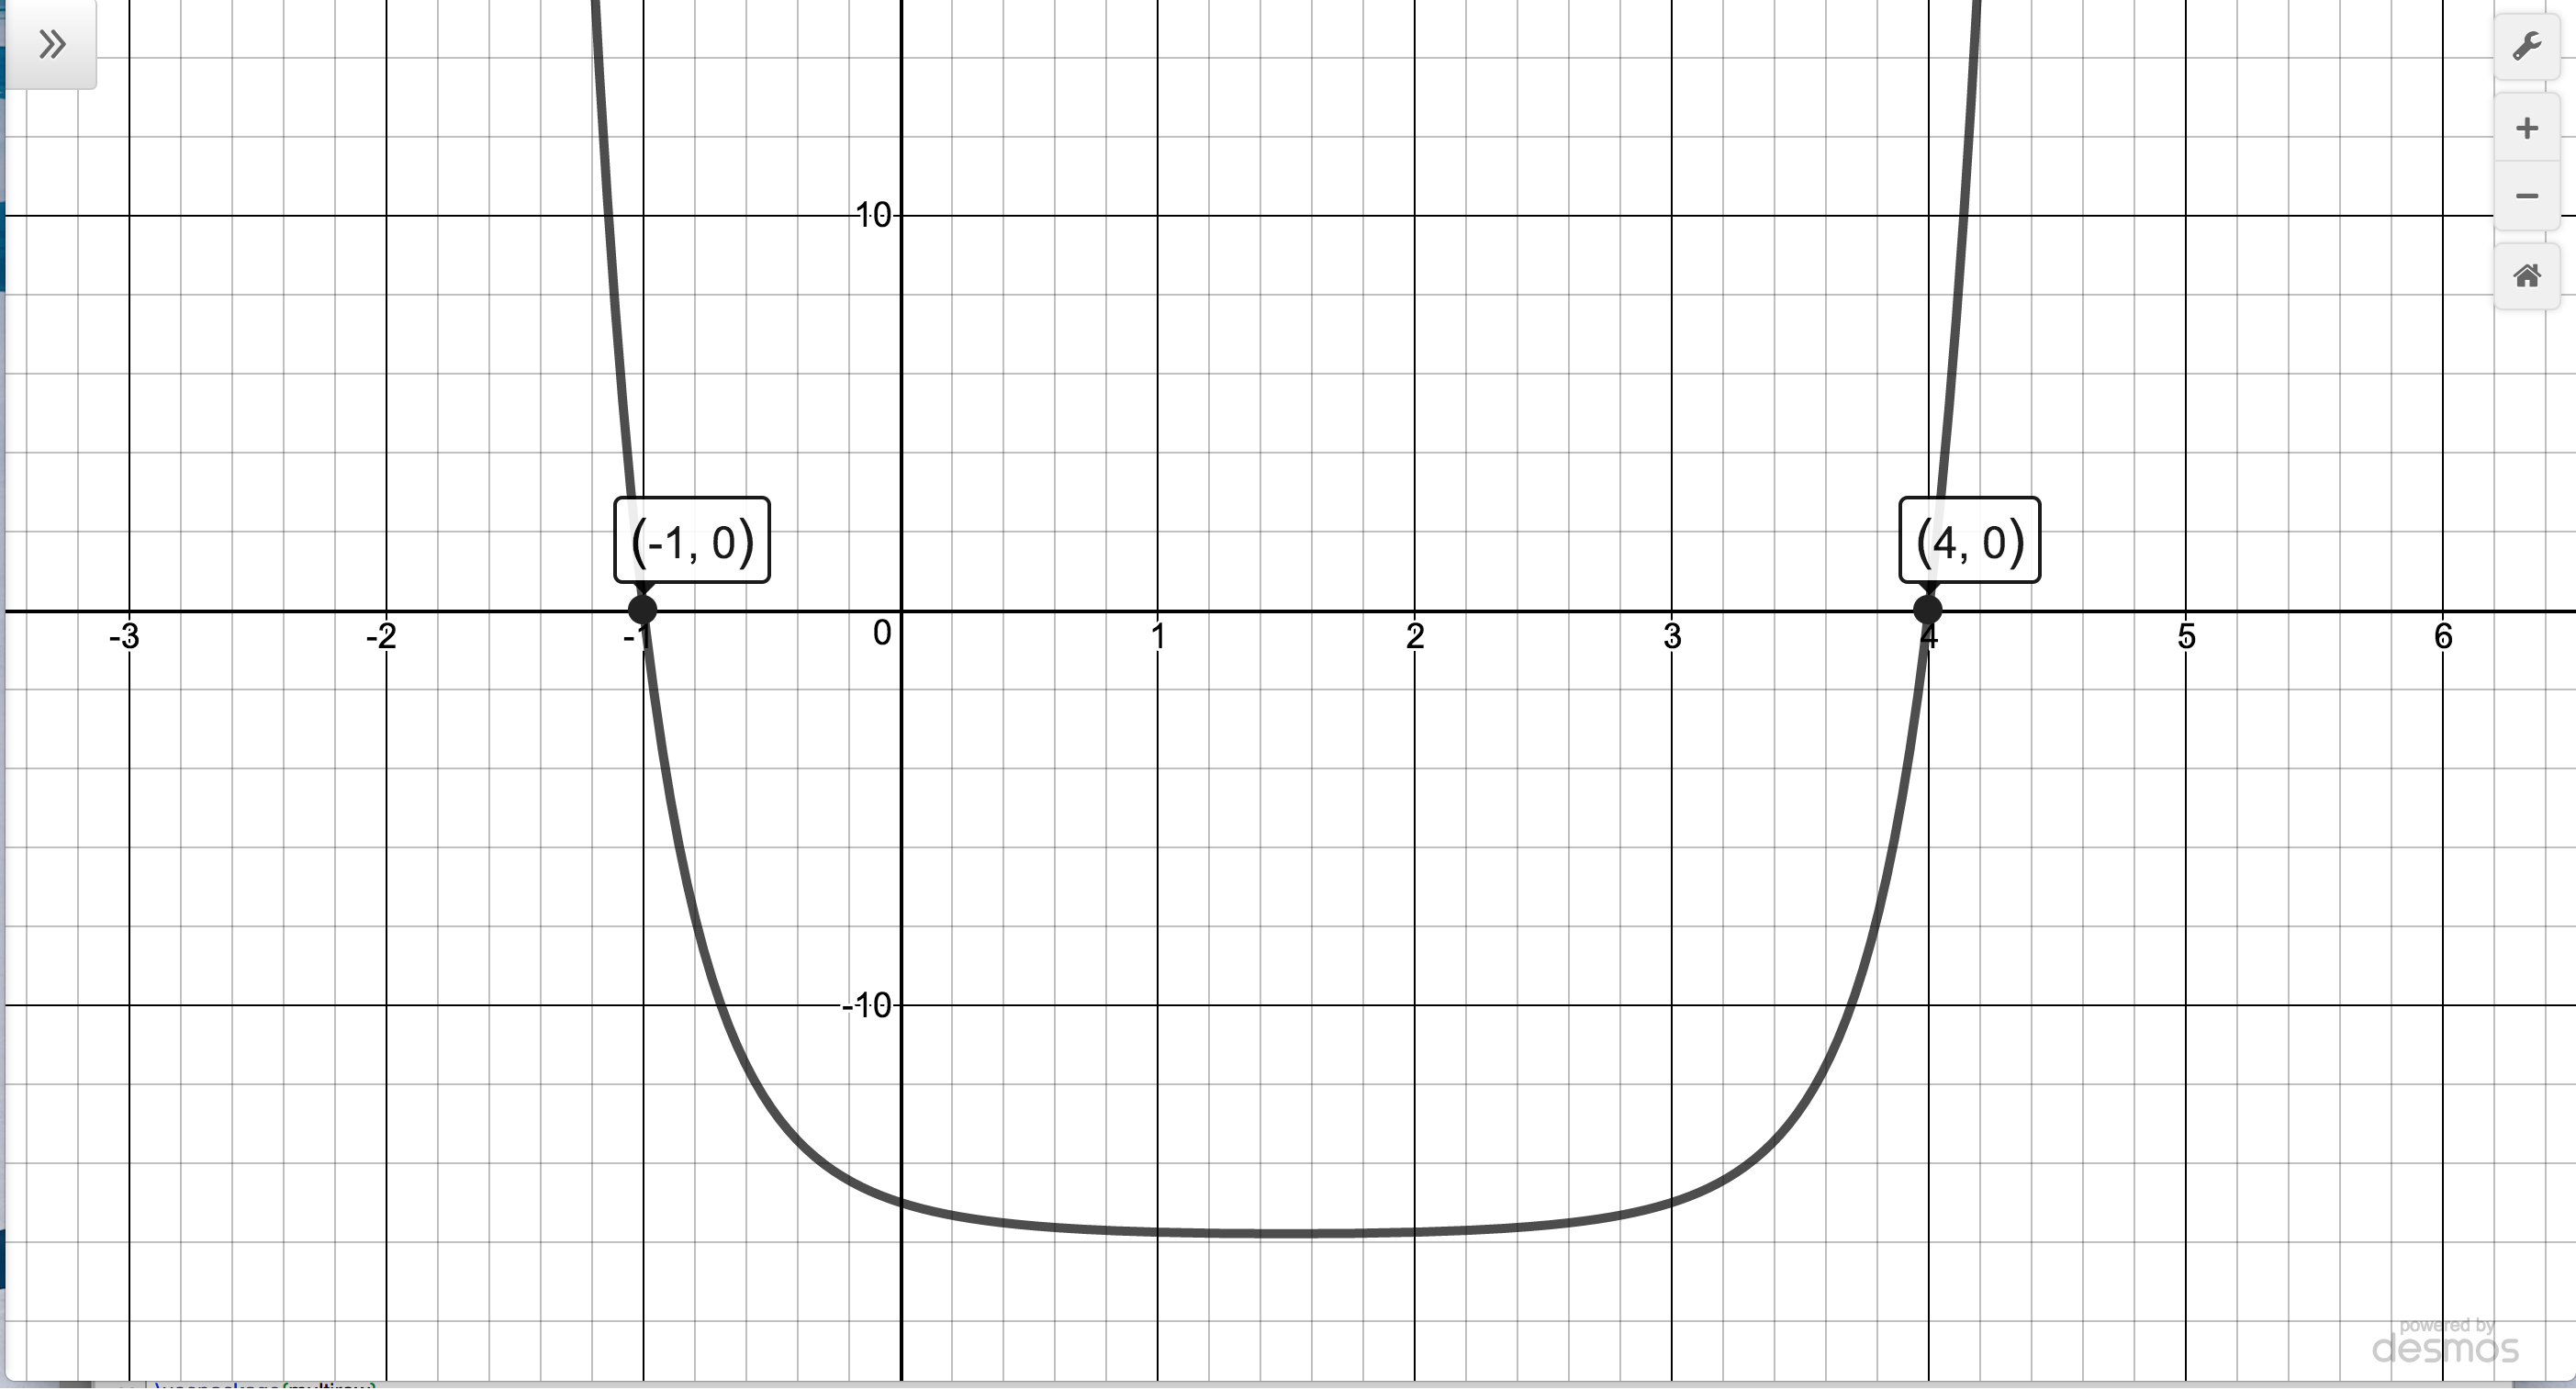
\includegraphics[width=3in]{./ExponentialEquationsandInequalitiesGraphics/ExpEqnEx07.jpg}  \\
 
 
A Sign Diagram for  $r(x) = 2^{x^2-3x} - 16$ & 

Checking $2^{x^2-3x} - 16 \geq 0$ \\

\end{tabular}

\end{center}

\item The first step we need to take to solve  $\frac{e^{x}}{e^{x}-4} \leq 3$ is to get $0$ on one side of the inequality. To that end, we subtract $3$ from both sides and get a common denominator


\setlength{\extrarowheight}{12pt}
\[ \begin{array}{rclr}

\dfrac{e^{x}}{e^{x}-4} & \leq & 3 & \\

\dfrac{e^{x}}{e^{x}-4} - 3 & \leq & 0 & \\

\dfrac{e^{x}}{e^{x}-4} - \dfrac{3 \left(e^{x}-4\right)}{e^{x}-4} & \leq & 0 & \mbox{Common denomintors.} \\

\dfrac{12 - 2e^{x}}{e^{x}-4} & \leq & 0 & \\

\end{array}\]
\setlength{\extrarowheight}{2pt}

We set $r(x) = \frac{12 - 2e^{x}}{e^{x}-4}$ and we note that $r$ is undefined when its denominator $e^{x}-4=0$, or when $e^{x} = 4$.  Solving this gives $x = \ln(4)$, so the domain of $r$ is $(-\infty, \ln(4)) \cup (\ln(4), \infty)$. 

\smallskip

To find the zeros of $r$, we solve $r(x) = 0$ and obtain $12 - 2e^{x} = 0$.  We find $e^{x} = 6$, or $x = \ln(6)$.  

\smallskip

When we build our sign diagram, finding test values may be a little tricky since we need to check values around $\ln(4)$ and $\ln(6)$.  

\smallskip

Recall that the function $\ln(x)$ is increasing\footnote{This is because the base of $\ln(x)$ is $e > 1$.  If the base $b$ were in the interval $0 < b < 1$, then $\log_{b}(x)$ would decreasing.} which means $\ln(3) < \ln(4) < \ln(5) < \ln(6) < \ln(7)$.  

\smallskip

To determine the sign of $r\left(\ln(3)\right)$, we remember that $e^{\ln(3)} = 3$ and get \[r\left(\ln(3)\right) = \frac{12 - 2e^{\ln(3)}}{e^{\ln(3)}-4} = \frac{12-2(3)}{3-4} = -6.\]  

We determine the signs of $r\left(\ln(5)\right)$ and $r\left(\ln(7)\right)$ similarly.\footnote{We could, of course, use the calculator, but what fun would that be?} From the sign diagram, we find our answer to be $(-\infty,\ln(4)) \cup [\ln(6), \infty)$.  


\smallskip

Using a graphing utility, we find the graph of $f(x) = \frac{e^{x}}{e^{x}-4}$ is below the graph of $g(x) = 3$ on $(-\infty,\ln(4)) \cup (\ln(6), \infty)$, and they intersect at $x  \approx 1.792 \approx  \ln(6)$.


\begin{center}

\begin{tabular}{cc}

\begin{mfpic}[10]{-5}{5}{-1}{2}
\arrow \reverse \arrow \polyline{(-5,0),(5,0)}
\xmarks{-2,2}
\tlabel[cc](-3.5,1){$(-)$}
\tlabel[cc](-2,-1){$\ln(4)$}
\tlabel[cc](-2,1){\textinterrobang}
\tlabel[cc](0,1){$(+)$}
\tlabel[cc](2,-1){$\ln(6)$}
\tlabel[cc](2,1){$0$}
\tlabel[cc](3.5,1){$(-)$}
\end{mfpic}

& 

 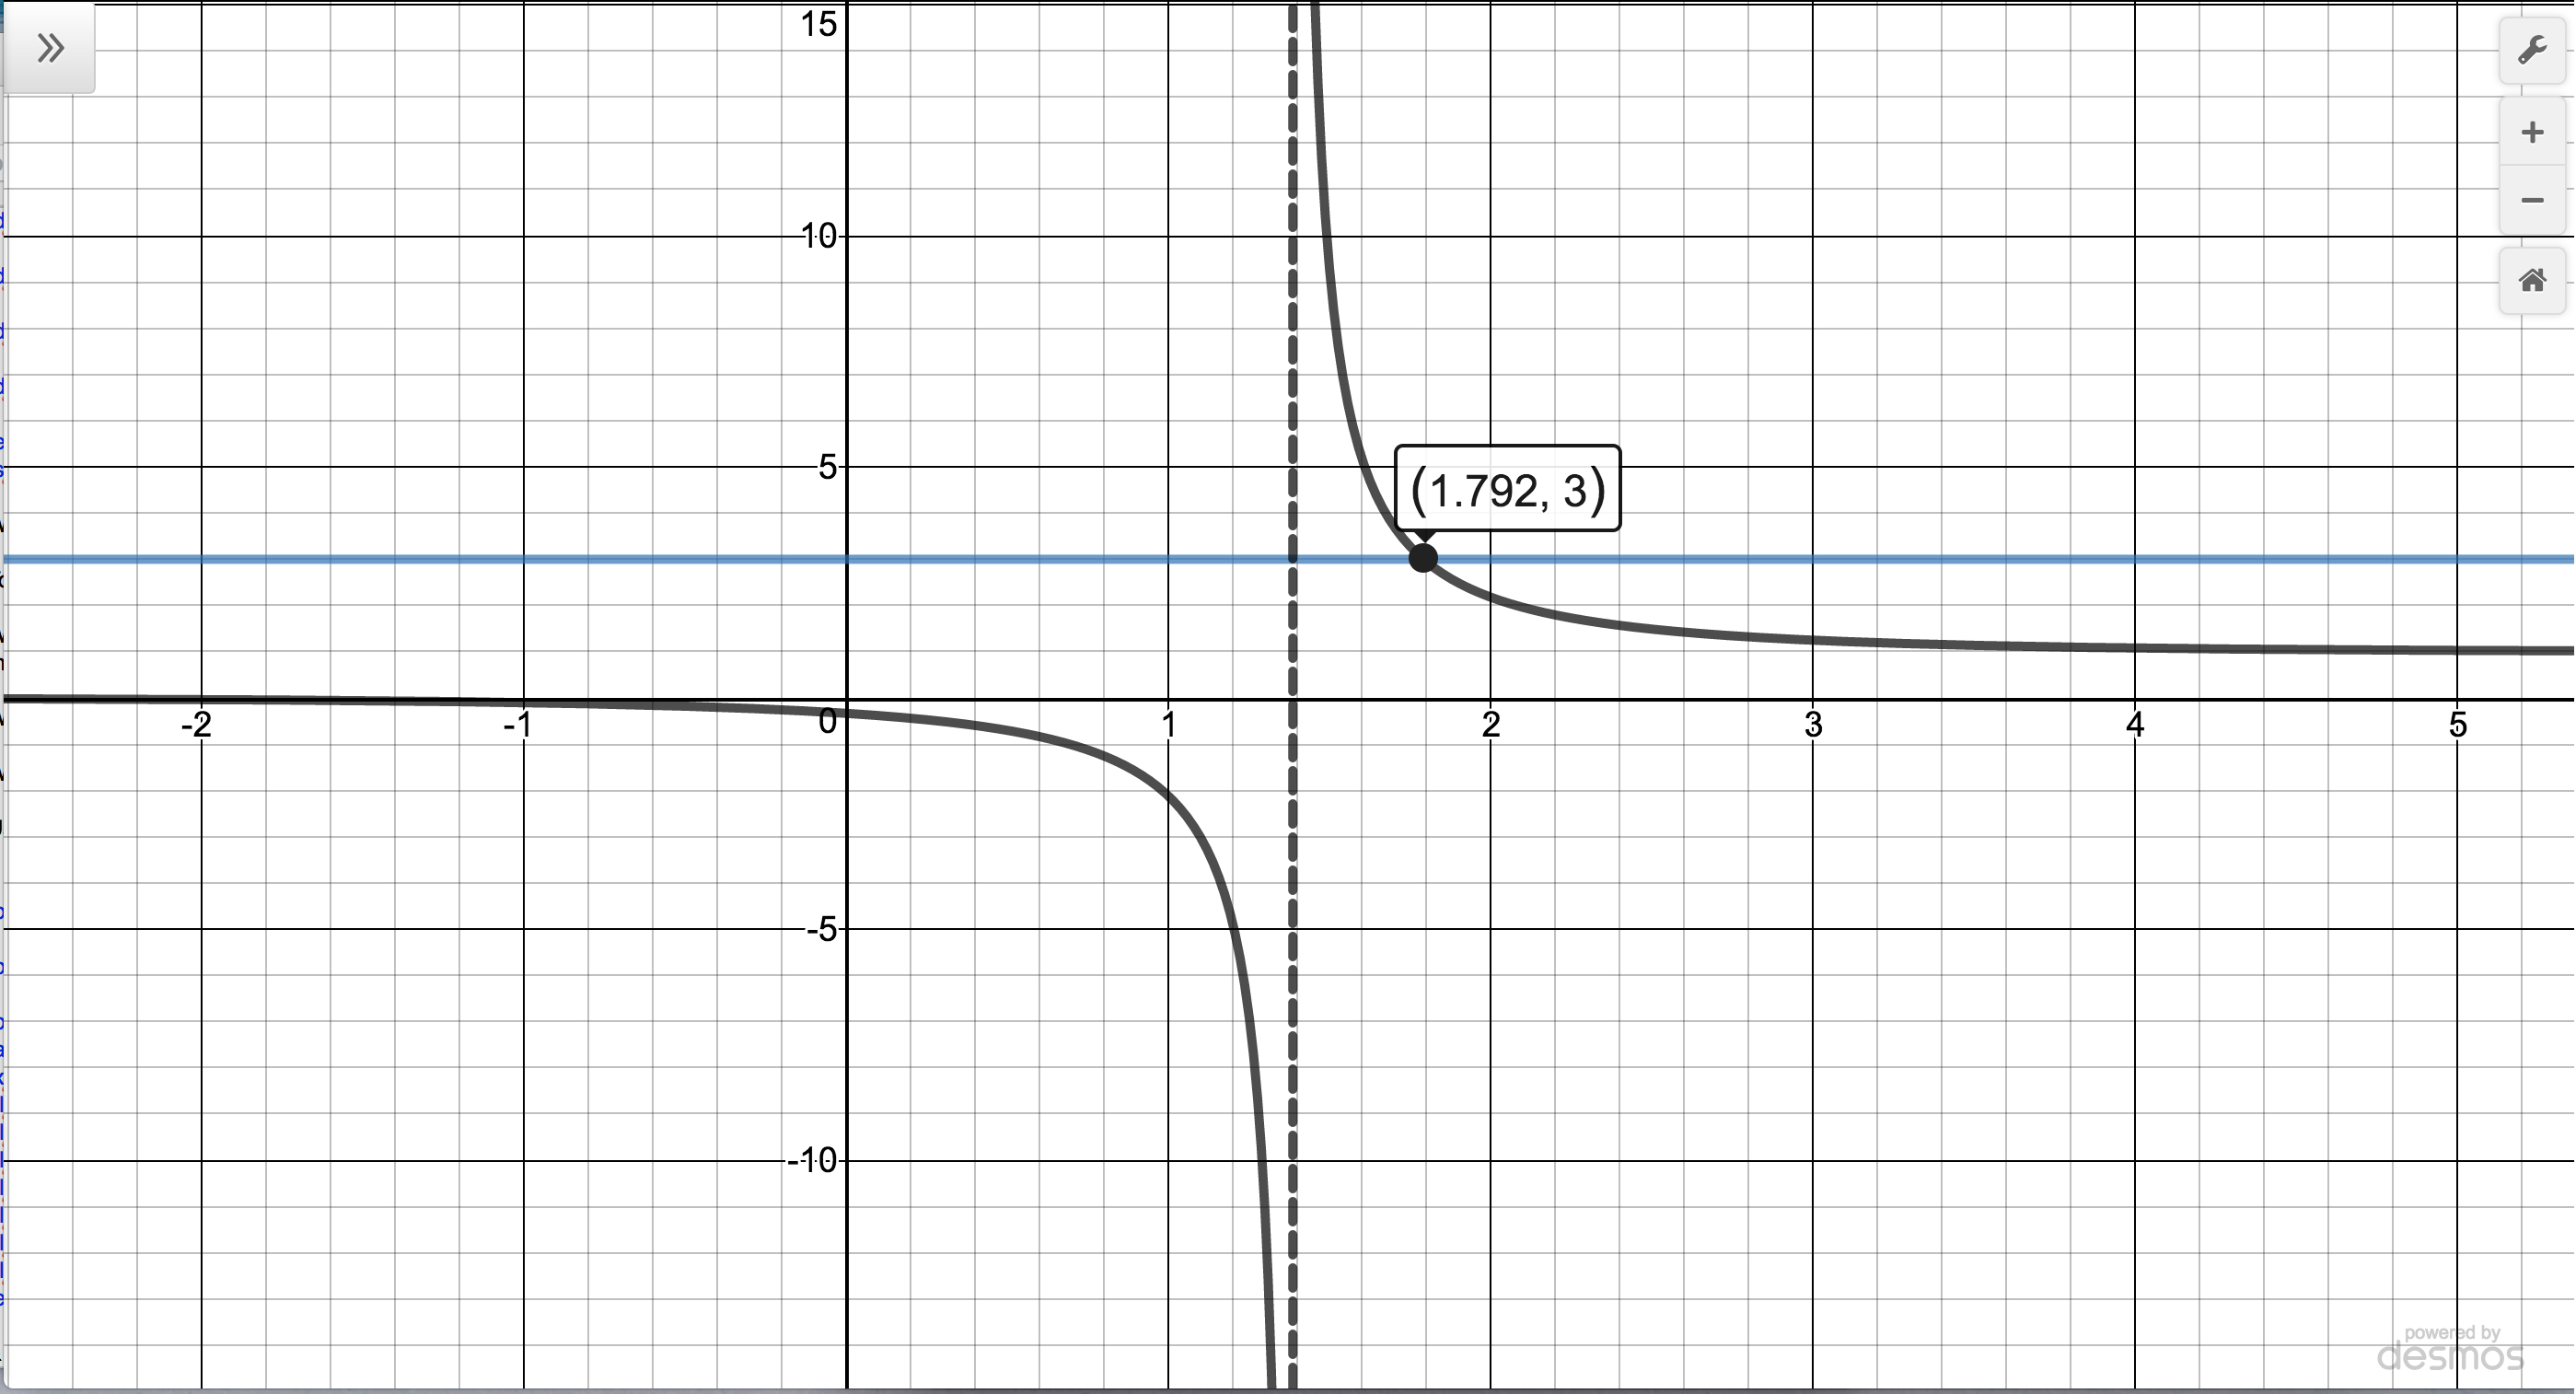
\includegraphics[width=3in]{./ExponentialEquationsandInequalitiesGraphics/ExpEqnEx08.jpg}  \\
 
 A Sign Diagram for  $r(x) = \dfrac{12 - 2e^{x}}{e^{x}-4}$ & 

Checking $\dfrac{e^{x}}{e^{x}-4} \leq 3$ \\

\end{tabular}

\end{center}


\item  As before, we start solving $t e^{2t} < 4t$ by getting $0$ on one side of the inequality, $t e^{2t} - 4t < 0$.   

\smallskip

We set $r(t) = te^{2t} - 4t$ and since there are no denominators, even-indexed radicals, or logs, the domain of $r$ is all real numbers.  

\smallskip

Setting $r(t) = 0$  produces $t e^{2t} - 4t  = 0$. We factor to get $t \left(e^{2t} - 4\right)  = 0$ which gives $t=0$ or $e^{2t} - 4 = 0$.  

\smallskip

To solve the latter, we isolate the exponential and take logs to get $2t = \ln(4)$, or $t = \frac{\ln(4)}{2}$ which simplifies to $t = \ln(2)$.  (Can you see why?)  

\smallskip

As in the previous example, we need to be careful about choosing test values.  Since $\ln(1) = 0$, we choose $\ln\left(\frac{1}{2}\right)$, $\ln\left(\frac{3}{2}\right)$ and $\ln(3)$.  Evaluating,\footnote{A calculator can be used at this point. As usual, we proceed without apologies, with the analytical method.} we get 

\[\begin{array}{rclr}

r\left(\ln\left(\frac{1}{2}\right)\right) & = & \ln\left(\frac{1}{2}\right) e^{2\ln\left(\frac{1}{2}\right)} - 4\ln\left(\frac{1}{2}\right) & \\

&= & \ln\left(\frac{1}{2}\right)e^{\ln\left(\frac{1}{2}\right)^2}- 4\ln\left(\frac{1}{2}\right) & \text{Power Rule} \\

& = & \ln\left(\frac{1}{2}\right)e^{\ln\left(\frac{1}{4}\right)}- 4\ln\left(\frac{1}{2}\right) & \\

& = & \frac{1}{4}  \ln\left(\frac{1}{2}\right) - 4  \ln\left(\frac{1}{2}\right) =  -\frac{15}{4} \ln\left(\frac{1}{2}\right) & \end{array}\] 

Since $\frac{1}{2} < 1$, $ \ln\left(\frac{1}{2}\right) < 0$ and we get $r(\ln\left(\frac{1}{2}\right))$ is $(+)$.  Proceeding similarly, we find $r\left(\ln\left(\frac{3}{2}\right)\right)  < 0$ and $r(\ln(3)) > 0$.  Our solution corresponds to $r(t) < 0$ which occurs on $(0 ,\ln(2))$.  

\smallskip

The graphing utility confirms that the graph of $f(t) = t e^{2t} $ is below the graph of $g(t) = 4t$ on $(0 ,\ln(2))$.\footnote{Note: $\ln(2) \approx 0.693$.}


\begin{center}

\begin{tabular}{cc}

\begin{mfpic}[10]{-5}{5}{-1}{2}
\arrow \reverse \arrow \polyline{(-5,0),(5,0)}
\xmarks{-2,2}
\tlabel[cc](-3.5,1){$(+)$}
\tlabel[cc](-2,-1){$0$}
\tlabel[cc](-2,1){0}
\tlabel[cc](0,1){$(-)$}
\tlabel[cc](2,-1){$\ln(2)$}
\tlabel[cc](2,1){$0$}
\tlabel[cc](3.5,1){$(+)$}
\end{mfpic}

& 

 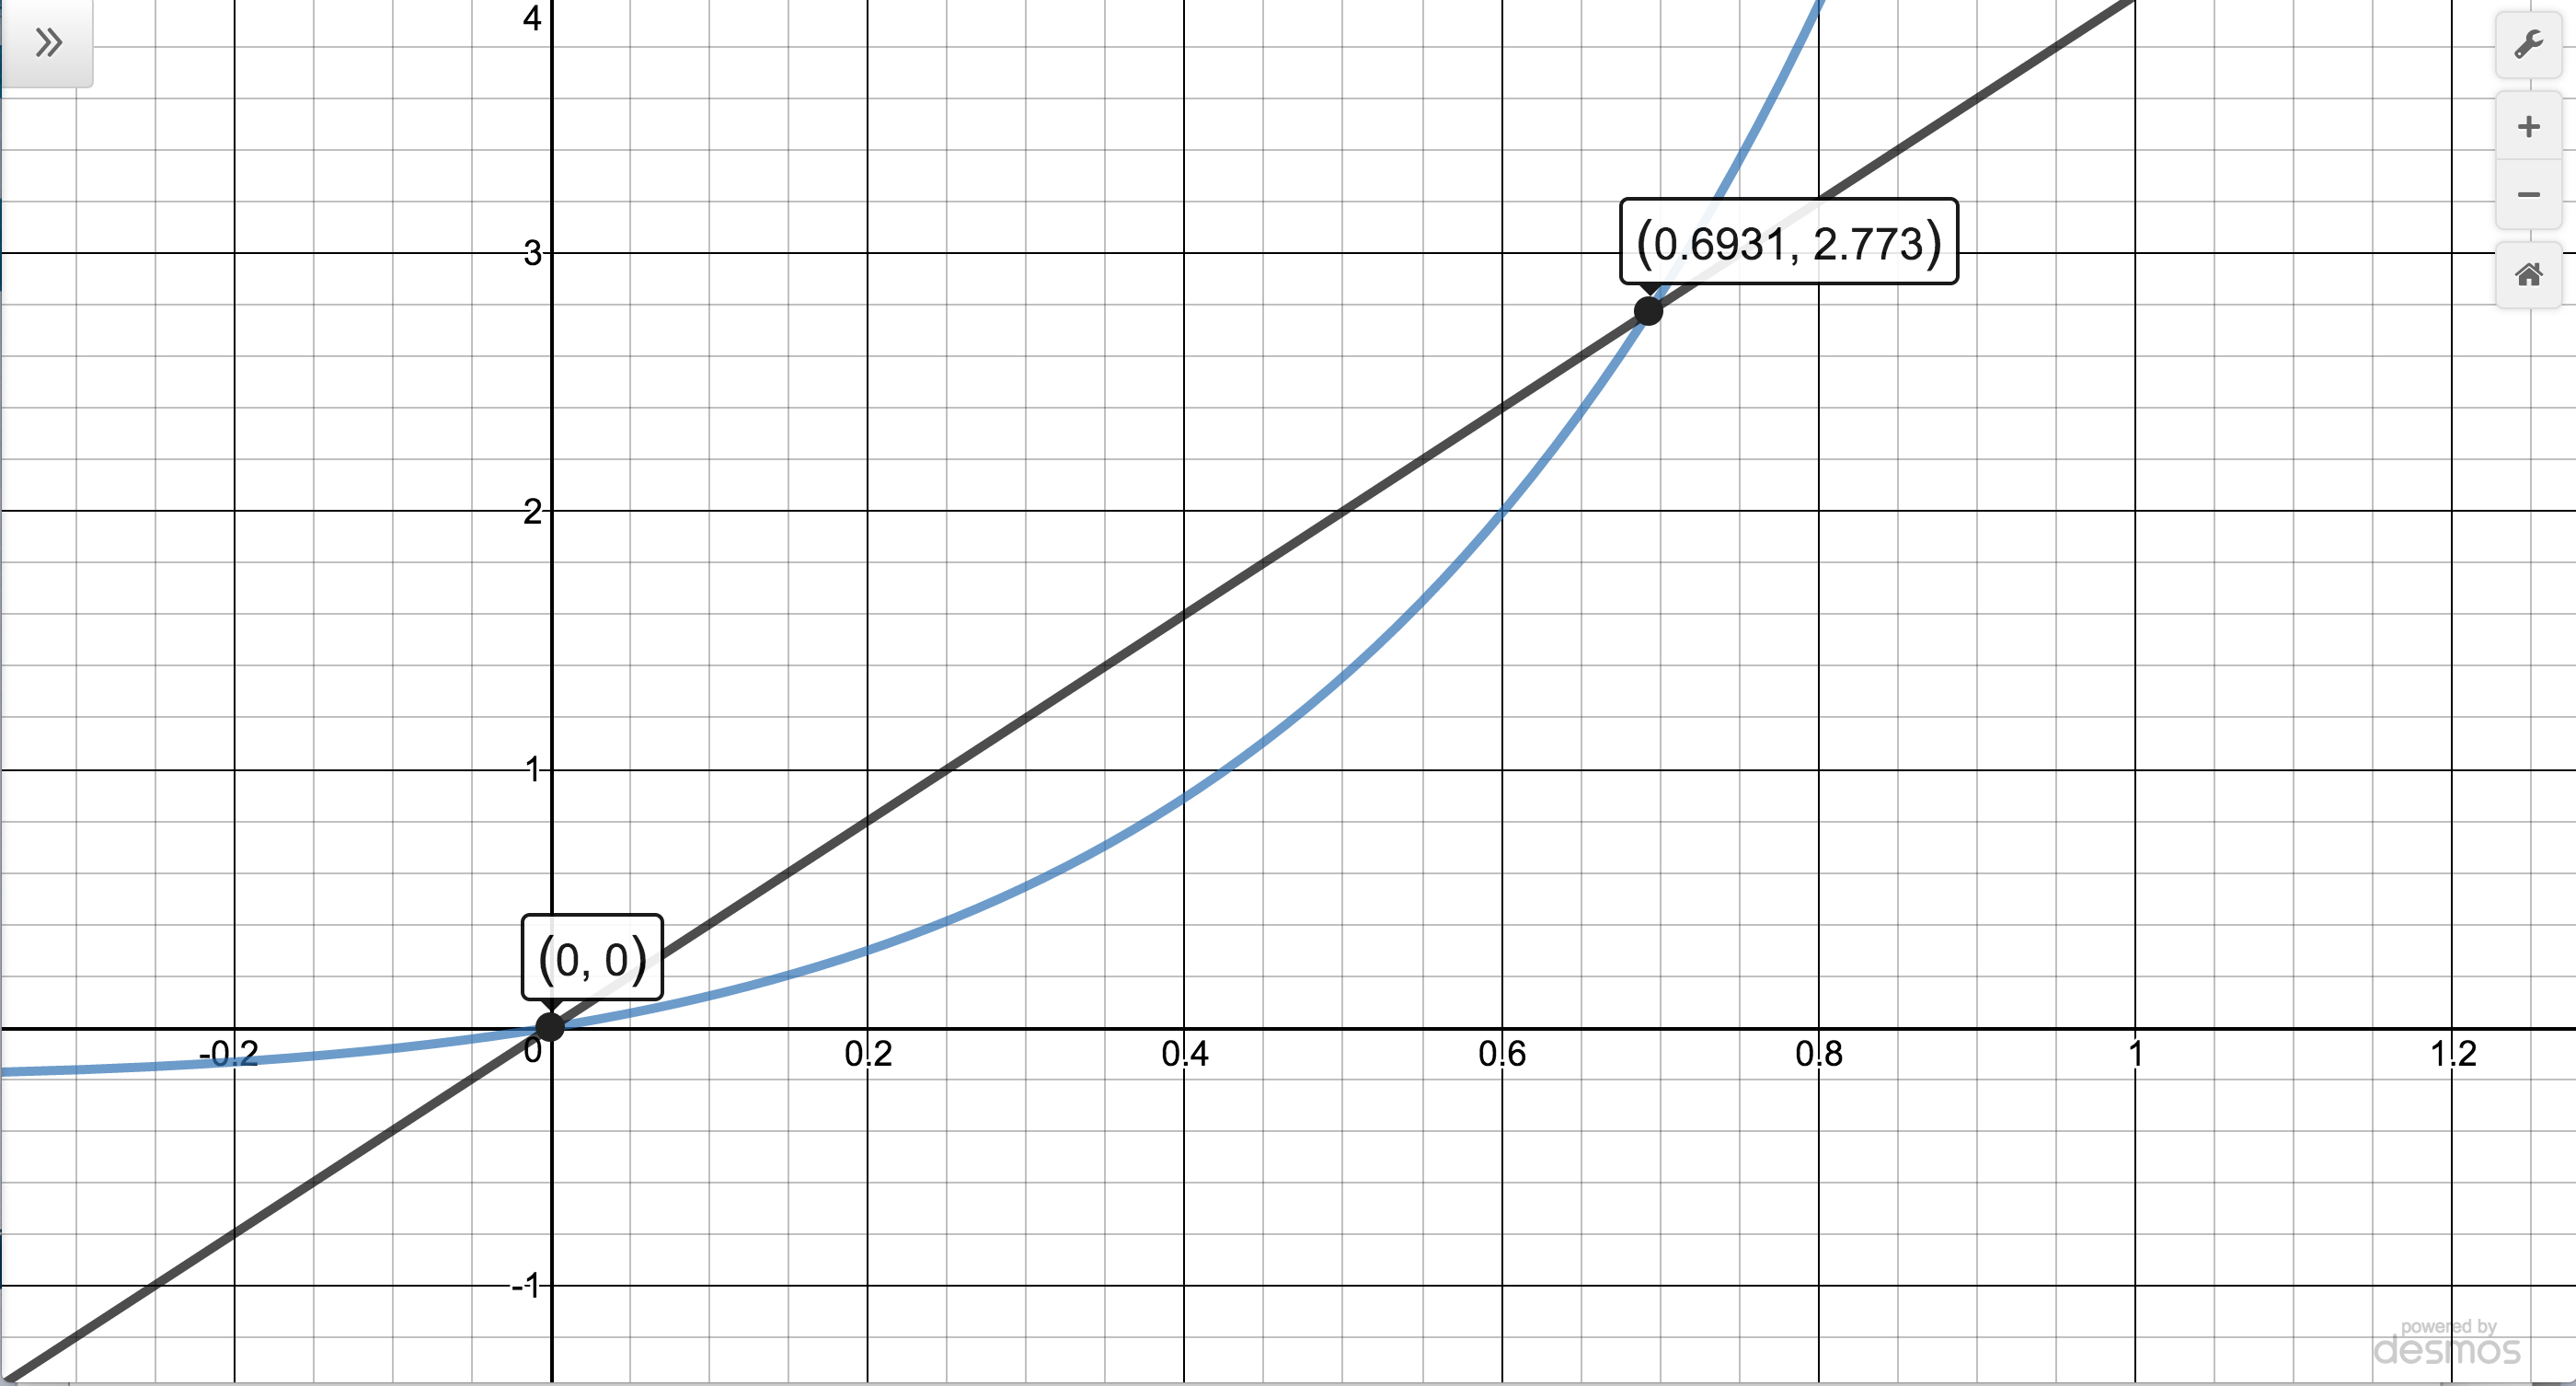
\includegraphics[width=3in]{./ExponentialEquationsandInequalitiesGraphics/ExpEqnEx09.jpg}  \\
 
 A Sign Diagram for  $r(t) = te^{2t} - 4t$  & 

Checking $t e^{2t} < 4t$ \\

\end{tabular}

\end{center}

\end{enumerate}

\qed

\end{ex}

We note here that while sign diagrams will \textit{always} work for solving inequalities involving exponential functions, as we've seen previously, there are circumstances in which we can short-cut this method. 

\smallskip

For example, consider number \ref{canuselogsex} from Example \ref{expineq} above:  $2^{x^2-3x} - 16 \geq 0$.  Since the base $2>1$, $\log_{2}(x)$ is an \textit{increasing} function meaning it preserves inequalities.

\smallskip

We can use this to our advantage in this case and eliminate the exponential from the inequality altogether:

\[ \begin{array}{rclr}

2^{x^2-3x} - 16 &  \geq &  0 &  \\

2^{x^2-3x}  & \geq & 16 & \\

\log_{2}\left(2^{x^2-3x} \right) & \geq & \log_{2}(16) & \text{$f(x) = \log_{2}(x)$ is increasing so if $b \geq a$, $\log_{2}(b) \geq \log_{2}(a)$. } \\

x^2 - 3x & \geq & 4 &\\ \end{array} \]

Hence, we've  reduced our given inequality to $x^2-3x \geq 4$.  As seen in Section \ref{QuadraticFunctions}, we can solve this inequality by completing the square, graphing, or a sign diagram, whichever strikes the reader's fancy.

\smallskip

Our next example is a follow-up to Example \ref{exptempex} in Section \ref{ExponentialFunctions}.  

\smallskip

\begin{ex}  \label{coffeewarmerex} Recall from Example \ref{exptempex}  the temperature of coffee $T$ (in degrees Fahrenheit) $t$ minutes after it is served can be modeled by $T(t) = 70 + 90 e^{-0.1 t}$.  When will the coffee be warmer than $100^{\circ}\mbox{F}$?

\smallskip

{\bf Solution.}  We need to find when $T(t) > 100$, that is, we need to solve  $70 + 90 e^{-0.1 t} > 100$.  

\smallskip

To use a sign diagram, we need to get $0$ on one side of the inequality.  Subtracting $100$ from both sides of $70 + 90 e^{-0.1 t} > 100$ produces   $90 e^{-0.1 t} - 30 > 0$. 

\smallskip

Identifying  $r(t) = 90 e^{-0.1 t} - 30$, we note from the context of the problem the domain of $r$ is $[0, \infty)$, so to build the sign diagram, we proceed to find the zeros of $r$.  

\smallskip

Solving $90 e^{-0.1 t} - 30=0$ results in $e^{-0.1t} = \frac{1}{3}$ so that $t = -10\ln\left(\frac{1}{3}\right)$  which reduces to $t = 10 \ln(3)$.

\smallskip

If we wish to avoid using the calculator to choose test values, we note that $f(x)  = \ln(x)$ is increasing.  As a result,  since $1 < 3$, $0 = \ln(1) < \ln(3)$ which proves $10\ln(3) > 0$. Hence, we may choose $t = 0$ as a test value in $[0, 10 \ln(3))$.  Since $3 < 4$, $\ln(3) < \ln(4)$, so $10 \ln(3) < 10 \ln(4)$. Hence,  we may choose $10 \ln(4)$   as test value for the interval $(10 \ln(3), \infty)$. 

\smallskip

We find $r(0)>0$ and $r(10\ln(4))<0$  which gives  the sign diagram below. We see $r(t)>0$ on $[0, 10\ln(3))$.

\smallskip

We graph $y=T(t)$ from Example  \ref{exptempex} below on the right along with with the horizontal line $y = 100$.   We see the graph of $T$ is above the horizontal line to the left of the intersection point, which we leave to the reader to show is $(10 \ln(3), 100)$.

\begin{center}

\begin{tabular}{m{0.5in}m{2.5in}m{2.5in}}

&

\begin{mfpic}[10]{0}{8}{-2}{2}
\arrow \polyline{(0,0), (8,0)}
\xmarks{0,4}
\tlabel[cc](0,-1){$0$}
\tlabel[cc](0,1){$(+)$}
\tlabel[cc](4,-1){ $10 \ln(3)$}
\tlabel[cc](4,1){$0$}
\tlabel[cc](6,1){$(-)$}
\end{mfpic}

& 

\begin{mfpic}[15]{-1}{11}{-1}{10}
\point[2pt]{(0,8)}
\dashed \polyline{(-1,3.5),(11,3.5)}
\axes
\tlabel[cc](9,3){\scriptsize H.A. $y=70$}
\tlabel[cc](9,5.5){\scriptsize $y=100$}
\tlabel[cc](11,-0.5){\scriptsize $t$}
\tlabel[cc](0.5,10){\scriptsize $y$}
\tcaption{\scriptsize $y = T(t)$}
\ymarks{1,2,3,4,5,6,7,8,9}
\xmarks{1,2,3,4,5,6,7,8,9,10}
\tlpointsep{4pt}
\axislabels {x}{{\scriptsize $2$} 1, {\scriptsize $4$} 2, {\scriptsize $6$} 3, {\scriptsize $8$} 4,{\scriptsize $10$} 5, {\scriptsize $12$} 6, {\scriptsize $14$} 7, {\scriptsize $16$} 8, {\scriptsize $18$} 9, {\scriptsize $20$} 10}
\axislabels {y}{{\scriptsize $20$} 1, {\scriptsize $40$} 2, {\scriptsize $60$} 3,{\scriptsize $80$} 4, {\scriptsize $120$} 6,{\scriptsize $140$} 7, {\scriptsize $160$} 8, {\scriptsize $180$} 9}
\penwd{1.25pt}
\arrow \reverse \arrow \polyline{(-1,5),(11,5)}
\arrow \function{0, 10, 0.1}{(90*exp(0-0.2*x)+70)/20}
\point[4pt]{(0,8), (5.5,5)}
\end{mfpic} \\

\end{tabular}

\end{center}

Hence, the coffee is warmer than $100^{\circ}$F up to $10 \ln(3) \approx 11$ minutes after it is served, or, said differently, it takes approximately 11 minutes for the coffee to cool to under $100^{\circ}$F.  \qed

\end{ex}

We note that, once again, we can short-cut the sign diagram in Example \ref{coffeewarmerex} to solve $70 + 90 e^{-0.1 t} > 100$.  Since $\ln(x)$ is increasing, it preserves inequality.  This means we can solve this inequality as follows.

\[ \begin{array}{rclr}

70 + 90 e^{-0.1 t} & > & 100 & \\
90 e^{-0.1 t} & > & 30 & \\
e^{-0.1 t} > & \frac{1}{3} & \\
\ln \left( e^{-0.1 t} \right) & > & \ln \left( \frac{1}{3} \right) & \text{$f(x) = \ln(x)$ is increasing so if $b \geq a$, $\ln(b) \geq  \ln(a)$. } \\
-0.1 t & > & - \ln(3) & \text{$\ln \left( \frac{1}{3} \right) = \ln \left(3^{-1} \right) = - \ln(3)$.} \\
t & < & \frac{-\ln(3)}{-0.1} = 10 \ln(3) & \\ \end{array} \]

Since we are given $t \geq 0$, we arrive at the same answer $0 \leq t < 10\ln(3)$ or $[0, 10 \ln(3))$.  

\smallskip

Note the importance, once again, of having a base larger than $1$ so that the corresponding logarithmic function is \textit{increasing}.  We can still adapt this strategy to exponential functions whose base is less than $1$, but we need to remember the corresponding logarithmic function is \textit{decreasing} so it \textit{reverses}  inequalities.  


\newpage

\begin{ex}  \label{expfracinverse} The function $f(x) = \dfrac{5e^{x}}{e^{x}+1}$ is one-to-one. 

\begin{multicols}{2} 

\begin{enumerate}

\item Find a formula for $f^{-1}(x)$.

\item  Solve $\dfrac{5e^{x}}{e^{x}+1} = 4$.

\end{enumerate}

\end{multicols}

{\bf Solution.}  \begin{enumerate} \item We start by writing $y=f(x)$, and interchange the roles of $x$ and $y$.  To solve for $y$, we first clear denominators and then isolate the exponential function.

\[ \begin{array}{rclr}
y & = & \dfrac{5e^{x}}{e^{x}+1} & \\ [12pt]
x & = & \dfrac{5e^{y}}{e^{y}+1} & \mbox{Switch $x$ and $y$} \\ [12pt]
x \left(e^{y}+1\right) & = & 5e^{y} & \\ [4pt]
x e^{y}+x & = & 5e^{y} & \\ [4pt]
x & = & 5e^{y} - x e^{y} & \\ [4pt]
x & = & e^{y}(5 - x) & \\ [4pt]
e^{y}& = & \dfrac{x}{5-x} & \\[12pt]
\ln\left(e^{y}\right) & = & \ln\left(\dfrac{x}{5-x}\right) & \\[12pt]
y & = & \ln\left(\dfrac{x}{5-x}\right) & \\
\end{array}\]

We claim $f^{-1}(x) = \ln\left(\frac{x}{5-x}\right)$.  To verify this analytically, we would need to verify the compositions $\left(f^{-1} \circ f\right)(x) = x$ for all $x$ in the domain of $f$ and that $\left(f \circ f^{-1}\right)(x) = x$ for all $x$ in the domain of $f^{-1}$.   We leave this, as well as a graphical check, to the reader in Exercise \ref{checkingexpfracinverse}.

%To verify our solution graphically, we graph $y = f(x) = \frac{5e^{x}}{e^{x}+1}$ and $y = g(x) = \ln\left(\frac{x}{5-x}\right)$ on the same set of axes and observe the symmetry about the line $y=x$ below.
%\begin{center}

% 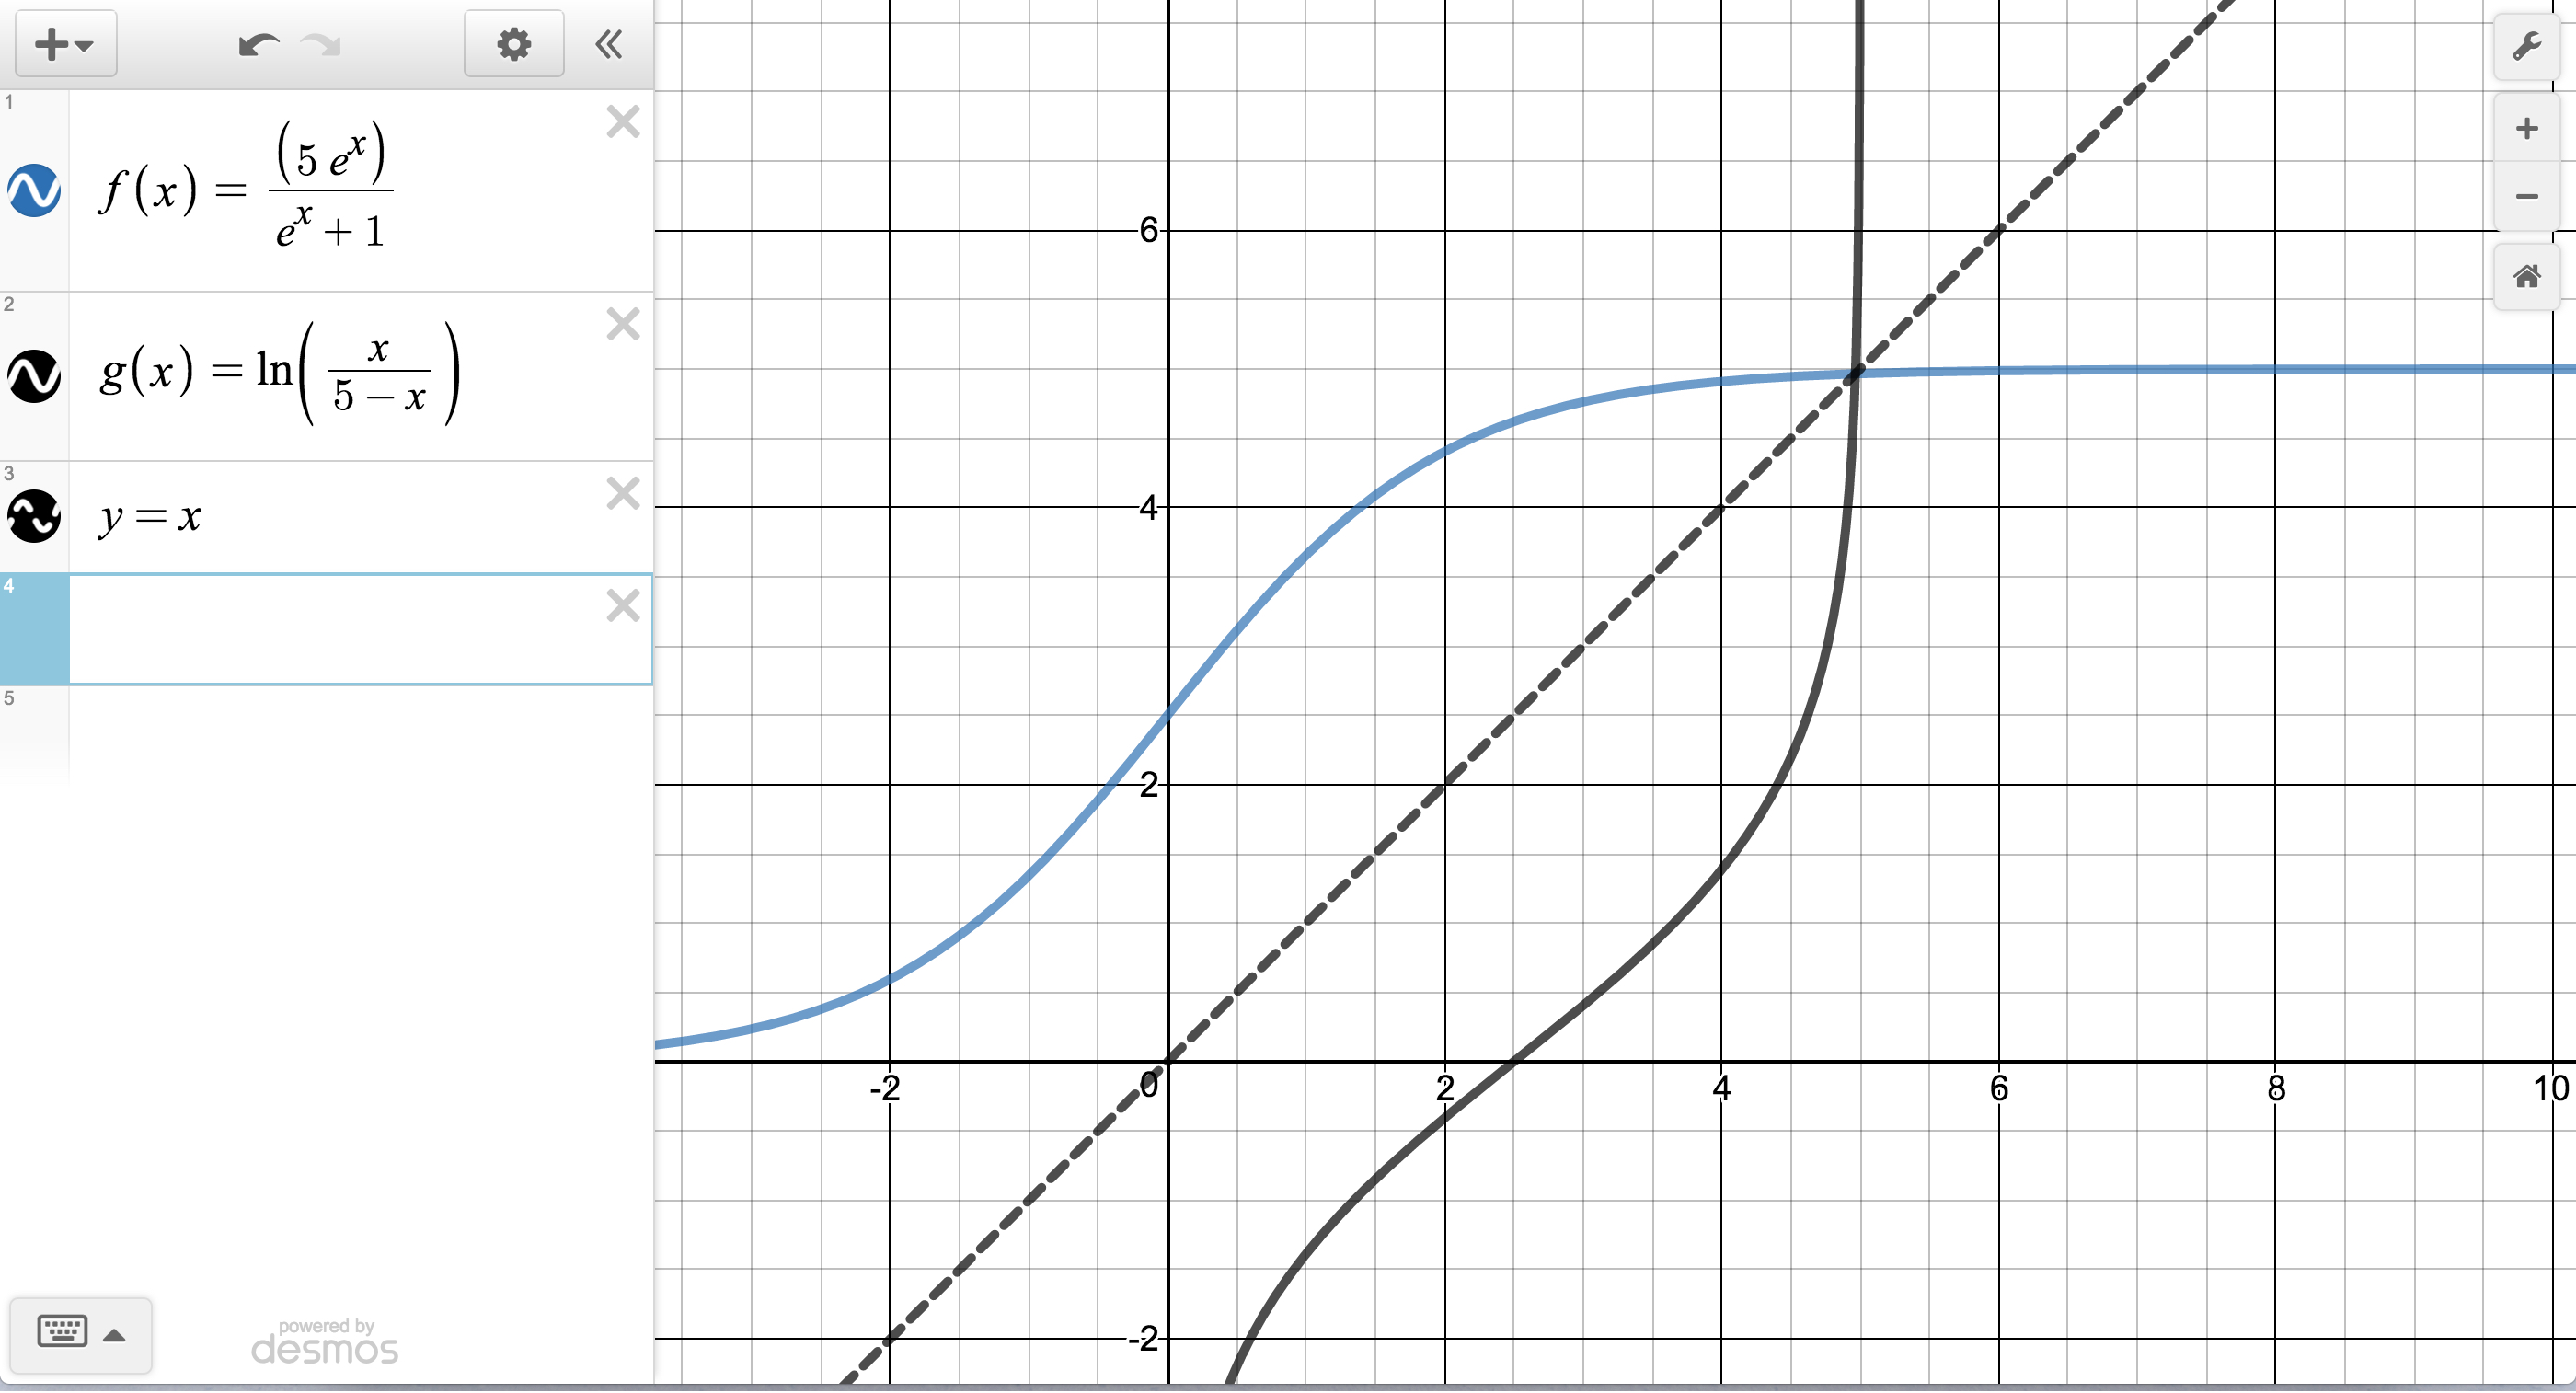
\includegraphics[width=4in]{./ExponentialEquationsandInequalitiesGraphics/ExpEqnEx10.jpg}

%\end{center}

\item We recognize the equation $\frac{5e^{x}}{e^{x}+1} = 4$ as $f(x) = 4$.  Hence, our solution is $x = f^{-1}(4) = \ln\left(\frac{4}{5-4}\right) = \ln(4)$.  

We can check this fairly quickly algebraically.  Using  $e^{\ln(4)} = 4$, we find $\frac{5e^{\ln(4)}}{e^{\ln(4)}+1}  = \frac{5(4)}{4+1} = \frac{20}{5} = 4$. \qed

\end{enumerate}

\end{ex}

\pagebreak

Our last example uses the tools of this section along with those developed in Section \ref{AppDerivatives}.

\begin{ex}\label{exponentialcurvesketchingex} Let $f(x) = 3xe^{-x}$.

\begin{enumerate}

\item  Given that $f'(x) = 3e^{-x} - 3x e^{-x}$, find the open intervals over which $f$ is increasing and decreasing.

\item Find the local extrema.\footnote{Recall this means the local maximums and minimums.}

\item Given that $f''(x) = 3xe^{-x} - 6e^{-x}$, find the open intervals over which the graph of $f$ is concave up and concave down.

\item  Locate the inflection points.

\item  Check your answers using a graphing utility.

\end{enumerate}

{\bf Solution.}

\begin{enumerate}

\item  To determine where $f$ is increasing and decreasing, we need to make a sign diagram for $f'(x)$.  Since the domain of $f'$ is all real numbers, we just need to find the zeros of $f'$. 

\medskip

Solving $f'(x) =  3e^{-x} - 3x e^{-x} = 0$ gives $3e^{-x} (1-x) = 0$ so $3e^{-x} = 0$, which has no solution,  or $1-x =0$ so $x=1$.  We make a sign diagram for $f'(x)$ below.

\begin{center}

\begin{multicols}{2}

\begin{mfpic}[10]{-6}{6}{-2}{2}
\arrow \reverse \arrow \polyline{(-5,0),(5,0)}
\xmarks{0}
\arrow \polyline{(-3,-1.5),(-3,-0.5)}
\arrow \polyline{(3,-1.5),(3,-0.5)}
\tlpointsep{4pt}
\axislabels {x}{{$1$} 0}
\tlabel[cc](-3,1){$(+)$}
\tlabel[cc](0,1){$0$}
\tlabel[cc](3,1){$(-)$}
\tlabel[cc](-3,-3.25){$0$}
\tlabel[cc](3,-3.25){$2$}
\tlabel[cc](6,1){$f'(x)$}
\tlabel[cc](6,-1){$x$}
%\tlabel[cc](6,0){$\infty$}
%\tlabel[cc](-6,0){$-\infty$}
\end{mfpic}

\begin{mfpic}[10]{-6}{6}{-2}{2}
\arrow \reverse \arrow \polyline{(-5,0),(5,0)}
\xmarks{0}
%\arrow \polyline{(-2,-1.5),(-2,-0.5)}
%\arrow \polyline{(2,-1.5),(2,-0.5)}
\tlpointsep{4pt}
\axislabels {x}{{$1$} 0}
\tlabel[cc](-3,1){$\nearrow$}
\tlabel[cc](0,1){$\rightarrow$}
\tlabel[cc](3,1){$\searrow$}
%\tlabel[cc](-2,-2.25){$0$}
%\tlabel[cc](2,-2.25){$2$}
\tlabel[cc](6,1){$f(x)$}
\tlabel[cc](6,-1){$x$}
%\tlabel[cc](6,0){$\infty$}
%\tlabel[cc](-6,0){$-\infty$}
\end{mfpic}


\end{multicols}
\end{center}

We get $f$ is increasing on $(-\infty, 1)$ and decreasing on $(1, \infty)$.

\medskip

\item Using the sign diagram for $f'(x)$, we see we have a local maximum at $(1, f(1)) = \left(1, 3e^{-1} \right)$.

\medskip

\item Once again, the domain of $f''$ is all real numbers, so our first step in constructing a sign diagram for $f''(x)$ is to find the zeros.

\medskip

Solving $f''(x) = 3xe^{-x} - 6e^{-x} = 0$ gives $3e^{-x}(x-2) = 0$ so either $3e^{-x} = 0$, which has no solution, or $x-2 = 0$, so $x = 2$. We make the sign diagram for $f''(x)$ below.


\begin{center}

\begin{multicols}{2}

\begin{mfpic}[10]{-6}{6}{-2}{2}
\arrow \reverse \arrow \polyline{(-5,0),(5,0)}
\xmarks{0}
\arrow \polyline{(-3,-1.5),(-3,-0.5)}
\arrow \polyline{(3,-1.5),(3,-0.5)}
\tlpointsep{4pt}
\axislabels {x}{{$2$} 0}
\tlabel[cc](-3,1){$(-)$}
\tlabel[cc](0,1){$0$}
\tlabel[cc](3,1){$(+)$}
\tlabel[cc](-3,-2.25){$0$}
\tlabel[cc](3,-2.25){$3$}
\tlabel[cc](6,1){$f''(x)$}
\tlabel[cc](6,-1){$x$}
%\tlabel[cc](6,0){$\infty$}
%\tlabel[cc](-6,0){$-\infty$}
\end{mfpic}

\begin{mfpic}[10]{-6}{6}{-2}{2}
\arrow \reverse \arrow \polyline{(-5,0),(5,0)}
\xmarks{0}
%\arrow \polyline{(-2,-1.5),(-2,-0.5)}
%\arrow \polyline{(2,-1.5),(2,-0.5)}
\tlpointsep{4pt}
\axislabels {x}{{$2$} 0}
\tlabel[cc](-3,1){\Huge $\frown$}
%\tlabel[cc](0,1){$\rightarrow$}
\tlabel[cc](3,1){\Huge $\smile$}
%\tlabel[cc](-2,-2.25){$0$}
%\tlabel[cc](2,-2.25){$2$}
\tlabel[cc](6,1){$f(x)$}
\tlabel[cc](6,-1){$x$}
%\tlabel[cc](6,0){$\infty$}
%\tlabel[cc](-6,0){$-\infty$}
\end{mfpic}


\end{multicols}
\end{center}

We see the graph of $f$ is concave up on $(-\infty, 2)$ and concave down on $(2, \infty)$.

\medskip

\item  Since $f$ changes concavity at $x=2$, we have an inflection point at $(2, f(2)) = \left( 2, 6e^{-2} \right)$.

\bigskip

\item We check using \href{https://www.desmos.com/calculator}{\underline{desmos}}:

\bigskip

\centerline{ 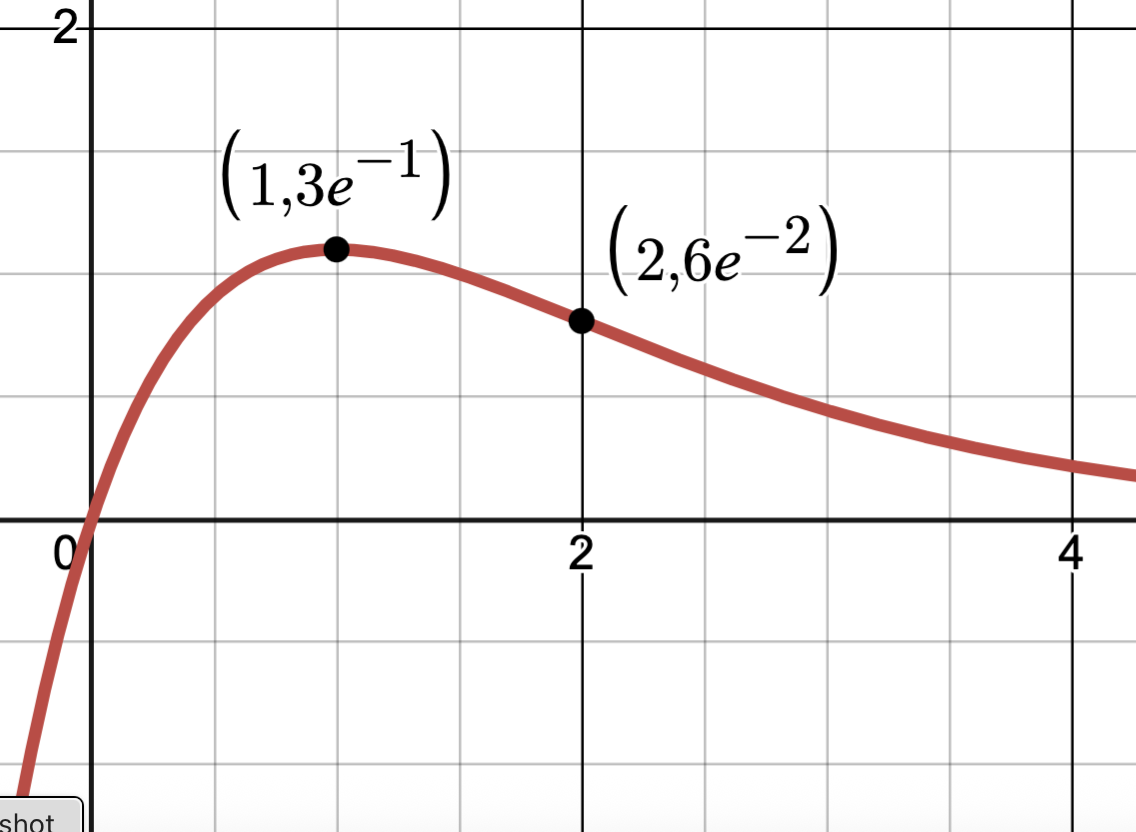
\includegraphics[width=3in]{./ExponentialEquationsandInequalitiesGraphics/ExpCurveSketchingExample.PNG}}

\hfill \qed

\end{enumerate}


\end{ex}

Note that the graph of $f(x) = 3xe^{-x}$ produced by the graphing utility in  Example \ref{exponentialcurvesketchingex} suggests the graph of $f$ has a horizontal asymptote as $x \rightarrow \infty$.

\medskip

Indeed, it is the case that $\ds{\lim_{x \rightarrow \infty} f(x) = 0}$, however if we try to reason this analytically, we get another instance of an indeterminate form.\footnote{Previously, we've seen the indeterminate form `$\frac{0}{0}$.'}  As $x \rightarrow \infty$, $3x \rightarrow \infty$ but $e^{-x} \rightarrow 0$.  Hence, as $x \rightarrow \infty$, we get the indeterminate form `$\infty \cdot 0$.' Depending on how quickly the first factor approaches `$\infty$' and how quickly the second factor approaches `$0$', we could end up with `$\infty$', `$0$,' or some number in between.\footnote{It is important here to understand that the factor  $e^{-x}$ which results in the `$0$' in the indeterminate form  `$\infty \cdot 0$' is \textbf{approaching} $0$ and is not actually \textbf{equal} to $0$.  An incorrect reasoning that  the form $\infty \cdot 0 \rightarrow 0$ in this case is that `anything times $0$ is $0$.'  Again, we'll have more to say about this in the Exercises.}

\medskip

We'll explore more of this phenomenon in Exercise \ref{powerexponentialgrowthex}.\footnote{With formal proofs found in Calculus \ldots} For now, we take it as true that exponential functions dominate polynomial functions so in the above indeterminate form,  the factor $e^{-x}$ determines\footnote{Less formally, the factor $e^{-x} \rightarrow 0$ `faster' than the factor $3x \rightarrow \infty$ which forces the product $3x e^{-x} \rightarrow 0$.} the end behavior of $f$, so $\ds{\lim_{x \rightarrow \infty} f(x) = 0}$.

\newpage

\subsection{Exercises}

%% SKIPPED %% \label{ExercisesforExponentialEquationsandInequalities}

In Exercises \ref{expeqnfirst} - \ref{expeqnlast}, solve the equation analytically.

\begin{multicols}{3}
\begin{enumerate}

\item $2^{4x} = 8$  \label{expeqnfirst} 
\item $3^{(x - 1)} = 27$  
\item $5^{2x-1} = 125$ 

\setcounter{HW}{\value{enumi}}
\end{enumerate}
\end{multicols}

\begin{multicols}{3}
\begin{enumerate}
\setcounter{enumi}{\value{HW}}

\item $4^{2t} = \frac{1}{2}$
\item $8^{t} = \frac{1}{128}$ 
\item $2^{(t^{3} - t)} = 1$ \vphantom{ $8^{t} = \frac{1}{128}$}

\setcounter{HW}{\value{enumi}}
\end{enumerate}
\end{multicols}

\begin{multicols}{3}
\begin{enumerate}
\setcounter{enumi}{\value{HW}}

\item $3^{7x} = 81^{4-2x}$ 
\item $9 \cdot 3^{7x} = \left(\frac{1}{9}\right)^{2x}$ 
\item $3^{2x} = 5$ 

\setcounter{HW}{\value{enumi}}
\end{enumerate}
\end{multicols}

\begin{multicols}{3}
\begin{enumerate}
\setcounter{enumi}{\value{HW}}

\item $5^{-t} = 2$ 
\item $5^{t} = -2$  
\item $3^{(t - 1)} = 29$  

\setcounter{HW}{\value{enumi}}
\end{enumerate}
\end{multicols}

\begin{multicols}{3}
\begin{enumerate}
\setcounter{enumi}{\value{HW}}

\item $(1.005)^{12x} = 3$
\item $e^{-5730k} = \frac{1}{2}$ 
\item $2000e^{0.1t} = 4000$  

\setcounter{HW}{\value{enumi}}
\end{enumerate}
\end{multicols}

\begin{multicols}{3}
\begin{enumerate}
\setcounter{enumi}{\value{HW}}


\item $500\left(1-e^{2t}\right) = 250$
\item $70 + 90e^{-0.1t} = 75$ 
\item $30-6e^{-0.1t}=20$ 


\setcounter{HW}{\value{enumi}}
\end{enumerate}
\end{multicols}

\begin{multicols}{3}
\begin{enumerate}
\setcounter{enumi}{\value{HW}}

\item $\dfrac{100e^{x}}{e^{x}+2}=50$ 
\item $\dfrac{5000}{1+2e^{-3t}}=2500$ 
\item $\dfrac{150}{1 + 29e^{-0.8t}} = 75$ 


\setcounter{HW}{\value{enumi}}
\end{enumerate}
\end{multicols}

\begin{multicols}{3}
\begin{enumerate}
\setcounter{enumi}{\value{HW}}

\item $25\left(\frac{4}{5}\right)^{x} = 10$  

\item $e^{2x} = 2e^{x}$ 
\item  $7e^{2t} = 28e^{-6t}$ 

\setcounter{HW}{\value{enumi}}
\end{enumerate}
\end{multicols}

\begin{multicols}{3}
\begin{enumerate}
\setcounter{enumi}{\value{HW}}

\item $3^{(x - 1)} = 2^{x}$ 
\item $3^{(x - 1)} = \left(\frac{1}{2}\right)^{(x + 5)}$ 
\item  $7^{3+7x} = 3^{4-2x}$  

\setcounter{HW}{\value{enumi}}
\end{enumerate}
\end{multicols}

\begin{multicols}{3}
\begin{enumerate}
\setcounter{enumi}{\value{HW}}

\item $e^{2t} - 3e^{t}-10=0$ %Ans $t=\ln(5)$
\item $e^{2t} = e^{t}+6$ %Ans $t=\ln(2)$
\item $4^{t} + 2^{t} = 12$ %Ans $x=\dfrac{\ln(3)}{\ln(2)}$


\setcounter{HW}{\value{enumi}}
\end{enumerate}
\end{multicols}

\begin{multicols}{3}
\begin{enumerate}
\setcounter{enumi}{\value{HW}}

\item $e^{x}-3e^{-x}=2$ %Ans $x=\ln(3)$
\item $e^{x}+15e^{-x}=8$ %Ans $x=\ln(2)$, $\ln(5)$
\item $3^{x}+25\cdot3^{-x}=10$ %Ans $x=\dfrac{\ln(5)}{\ln(3)}$
\label{expeqnlast} 

\setcounter{HW}{\value{enumi}}
\end{enumerate}
\end{multicols}

In Exercises \ref{expineqfirst} - \ref{expineqlast}, solve the inequality analytically.

\begin{multicols}{2} 
\begin{enumerate}
\setcounter{enumi}{\value{HW}}

\item $e^{x} > 53$ \label{expineqfirst} 
\item $1000\left(1.005\right)^{12t} \geq 3000$ 

\setcounter{HW}{\value{enumi}}
\end{enumerate}
\end{multicols}

\begin{multicols}{2} 
\begin{enumerate}
\setcounter{enumi}{\value{HW}}

\item $2^{(x^{3} - x)} < 1$
\item $25\left(\dfrac{4}{5}\right)^{x} \geq 10$

\setcounter{HW}{\value{enumi}}
\end{enumerate}
\end{multicols}

\begin{multicols}{2} 
\begin{enumerate}
\setcounter{enumi}{\value{HW}}

\item $\dfrac{150}{1 + 29e^{-0.8t}} \leq 130$

\item $\vphantom{\dfrac{150}{1 + 29e^{-0.8t}}} 70 + 90e^{-0.1t} \leq 75$

\setcounter{HW}{\value{enumi}}
\end{enumerate}
\end{multicols}

\begin{multicols}{2} 
\begin{enumerate}
\setcounter{enumi}{\value{HW}}

\item $e^{-x} - xe^{-x} \geq 0$
\item $(1-e^{t}) t^{-1} \leq 0$ \label{expineqlast}

\setcounter{HW}{\value{enumi}}
\end{enumerate}
\end{multicols}

In Exercises \ref{calcexpineqfirst} - \ref{calcexpineqlast},  use a graphing utility to help you solve the equation or  inequality.

\begin{multicols}{3} 
\begin{enumerate}
\setcounter{enumi}{\value{HW}}

\item $2^{x} = x^2$ \label{calcexpineqfirst} 
\item $e^{t} = \ln(t) + 5$   
\item $e^{\sqrt{x}} = x + 1$ 

\setcounter{HW}{\value{enumi}}
\end{enumerate}
\end{multicols}

\begin{multicols}{3} 
\begin{enumerate}
\setcounter{enumi}{\value{HW}}

\item  $e^{-2t}-te^{-t} \leq 0$
\item $3^{(x - 1)} < 2^{x}$ 
\item $e^{t} < t^{3} - t$ \label{calcexpineqlast} 

\setcounter{HW}{\value{enumi}}
\end{enumerate}
\end{multicols}

\pagebreak

In Exercises \ref{domaincomplicatedexpfirst} - \ref{domaincomplicatedexplast},  find the domain of the function.

\begin{multicols}{2} 
\begin{enumerate}
\setcounter{enumi}{\value{HW}}

\item  $T(x) = \dfrac{e^{x} - e^{-x}}{e^{x} + e^{-x}}$     \label{domaincomplicatedexpfirst}

\item   $C(x) = \dfrac{e^{x}  + e^{-x}}{e^{x}  - e^{-x}}$ 

\setcounter{HW}{\value{enumi}}
\end{enumerate}
\end{multicols}


\begin{multicols}{2} 
\begin{enumerate}
\setcounter{enumi}{\value{HW}}

\item     $s(t) = \sqrt{e^{2t} - 3}$
\item     $c(t) = \sqrt[3]{e^{2t} - 3}$

\setcounter{HW}{\value{enumi}}
\end{enumerate}
\end{multicols}

\begin{multicols}{2} 
\begin{enumerate}
\setcounter{enumi}{\value{HW}}
  
\item     $L(x) = \log\left( 3 - e^{x} \right)$  \vphantom{$\ell(x) = \ln\left( \dfrac{e^{2x}}{e^{x}-2} \right)$}

\item    $\ell(x) = \ln\left( \dfrac{e^{2x}}{e^{x}-2} \right)$  \label{domaincomplicatedexplast}

\setcounter{HW}{\value{enumi}}
\end{enumerate}
\end{multicols}




\begin{enumerate}
\setcounter{enumi}{\value{HW}}

\item \label{onetoonelogexercise} Since $f(x) = \ln(x)$ is a strictly increasing function, if $0 < a < b$ then $\ln(a) < \ln(b)$.  Use this fact to solve the inequality $e^{(3x - 1)} > 6$ without a sign diagram. Use this technique to solve the inequalities in Exercises \ref{expineqfirst} - \ref{expineqlast}. (NOTE:  Isolate the exponential function first!)

\item \label{hyperbolicsine} Compute the inverse of $f(x) = \dfrac{e^{x} - e^{-x}}{2}$.  State the domain and range of both $f$ and $f^{-1}$. 

\item \label{checkingexpfracinverse} In Example \ref{expfracinverse}, we found that the inverse of $f(x) = \dfrac{5e^{x}}{e^{x}+1}$ was $f^{-1}(x) = \ln\left(\dfrac{x}{5-x}\right)$ but we left a few loose ends for you to tie up.  

\begin{enumerate}

\item Algebraically check our answer by verifying: $\left(f^{-1} \circ f\right)(x) = x$ for all $x$ in the domain of $f$ and that $\left(f \circ f^{-1}\right)(x) = x$ for all $x$ in the domain of $f^{-1}$.

\item Find the range of $f$ by finding the domain of $f^{-1}$.

\item With help of a graphing utility, graph $y = f(x)$,  $y = f^{-1}(x)$ and $y = x$ on the same set of axes.  How does this help to verify our answer?

\item Let $g(x) = \dfrac{5x}{x+1}$ and $h(x) = e^{x}$.  Show that $f = g \circ h$ and that $(g \circ h)^{-1} = h^{-1} \circ g^{-1}$. 

NOTE:  We know this is true in general by Exercise \ref{fcircginverse} in Section \ref{InverseFunctions}, but it's nice to see a specific example of the property.

\end{enumerate}

\item With the help of your classmates, solve the inequality $e^{x} > x^{n}$ for a variety of natural numbers $n$.  What might you conjecture about the ``speed'' at which $f(x) = e^{x}$ grows versus any polynomial?

\end{enumerate}

\newpage

\subsection{Answers}


\begin{multicols}{3}
\begin{enumerate}

\item $x = \frac{3}{4}$
\item $x = 4$
\item $x=2$

\setcounter{HW}{\value{enumi}}
\end{enumerate}
\end{multicols}

\begin{multicols}{3}
\begin{enumerate}
\setcounter{enumi}{\value{HW}}

\item $t = -\frac{1}{4}$
\item $t = -\frac{7}{3}$
\item $t = -1, \, 0, \, 1$

\setcounter{HW}{\value{enumi}}
\end{enumerate}
\end{multicols}

\begin{multicols}{3}
\begin{enumerate}
\setcounter{enumi}{\value{HW}}

\item $x = \frac{16}{15}$
\item $x=-\frac{2}{11}$  \vphantom{$x = \dfrac{\ln(5)}{2\ln(3)}$}
\item $x = \dfrac{\ln(5)}{2\ln(3)}$

\setcounter{HW}{\value{enumi}}
\end{enumerate}
\end{multicols}

\begin{multicols}{3}
\begin{enumerate}
\setcounter{enumi}{\value{HW}}

\item $t = -\dfrac{\ln(2)}{\ln(5)}$
\item No solution. \vphantom{ $t = \dfrac{\ln(29) + \ln(3)}{\ln(3)}$}
\item $t = \dfrac{\ln(29) + \ln(3)}{\ln(3)}$

\setcounter{HW}{\value{enumi}}
\end{enumerate}
\end{multicols}

\begin{multicols}{3}
\begin{enumerate}
\setcounter{enumi}{\value{HW}}

\item $x = \dfrac{\ln(3)}{12\ln(1.005)}$ \vphantom{$k = \dfrac{\ln\left(\frac{1}{2}\right)}{-5730} = \dfrac{\ln(2)}{5730} $}
\item $k = \dfrac{\ln\left(\frac{1}{2}\right)}{-5730} = \dfrac{\ln(2)}{5730} $
\item $t=\dfrac{\ln(2)}{0.1} = 10\ln(2)$ \vphantom{$k = \dfrac{\ln\left(\frac{1}{2}\right)}{-5730} = \dfrac{\ln(2)}{5730} $}

\setcounter{HW}{\value{enumi}}
\end{enumerate}
\end{multicols}

\begin{multicols}{2}
\begin{enumerate}
\setcounter{enumi}{\value{HW}}


\item $t=\frac{1}{2}\ln\left(\frac{1}{2}\right) = -\frac{1}{2}\ln(2)$ \vphantom{$t = \dfrac{\ln\left(\frac{1}{18}\right)}{-0.1} =10 \ln(18)$}
\item $t = \dfrac{\ln\left(\frac{1}{18}\right)}{-0.1} =10 \ln(18)$

\setcounter{HW}{\value{enumi}}
\end{enumerate}
\end{multicols}

\begin{multicols}{2}
\begin{enumerate}
\setcounter{enumi}{\value{HW}}


\item $t=-10\ln\left(\frac{5}{3}\right) = 10\ln\left(\frac{3}{5}\right)$
\item$x=\ln(2)$ \vphantom{$t=-10\ln\left(\frac{5}{3}\right) = 10\ln\left(\frac{3}{5}\right)$}

\setcounter{HW}{\value{enumi}}
\end{enumerate}
\end{multicols}

\begin{multicols}{2}
\begin{enumerate}
\setcounter{enumi}{\value{HW}}

\item $t=\frac{1}{3}\ln(2)$ \vphantom{$t = \dfrac{\ln\left(\frac{1}{29}\right)}{-0.8} = \dfrac{5}{4}\ln(29)$}

\item $t = \dfrac{\ln\left(\frac{1}{29}\right)}{-0.8} = \dfrac{5}{4}\ln(29)$

\setcounter{HW}{\value{enumi}}
\end{enumerate}
\end{multicols}

\begin{multicols}{2}
\begin{enumerate}
\setcounter{enumi}{\value{HW}}

\item $x = \dfrac{\ln\left(\frac{2}{5}\right)}{\ln\left(\frac{4}{5}\right)} = \dfrac{\ln(2)-\ln(5)}{\ln(4) - \ln(5)}$

\item $x =  \ln(2)$ \vphantom{ $x = \dfrac{\ln\left(\frac{2}{5}\right)}{\ln\left(\frac{4}{5}\right)} = \dfrac{\ln(2)-\ln(5)}{\ln(4) - \ln(5)}$}


\setcounter{HW}{\value{enumi}}
\end{enumerate}
\end{multicols}

\begin{multicols}{2}
\begin{enumerate}
\setcounter{enumi}{\value{HW}}


\item  $t = -\frac{1}{8} \ln\left(\frac{1}{4} \right) = \frac{1}{4}\ln(2)$ \vphantom{$x = \dfrac{\ln(3)}{\ln(3) - \ln(2)}$}

\item $x = \dfrac{\ln(3)}{\ln(3) - \ln(2)}$

\setcounter{HW}{\value{enumi}}
\end{enumerate}
\end{multicols}

\begin{multicols}{2}
\begin{enumerate}
\setcounter{enumi}{\value{HW}}


\item $x = \dfrac{\ln(3) + 5\ln\left(\frac{1}{2}\right)}{\ln(3) - \ln\left(\frac{1}{2}\right)} = \dfrac{\ln(3)-5\ln(2)}{\ln(3)+\ln(2)}$
\item  $x = \dfrac{4 \ln(3) - 3 \ln(7)}{7 \ln(7) + 2 \ln(3)}$ \vphantom{$x = \dfrac{\ln(3) + 5\ln\left(\frac{1}{2}\right)}{\ln(3) - \ln\left(\frac{1}{2}\right)} = \dfrac{\ln(3)-5\ln(2)}{\ln(3)+\ln(2)}$}

\setcounter{HW}{\value{enumi}}
\end{enumerate}
\end{multicols}

\begin{multicols}{3}
\begin{enumerate}
\setcounter{enumi}{\value{HW}}

\item $t=\ln(5)$ \vphantom{$t=\dfrac{\ln(3)}{\ln(2)}$}
\item $t=\ln(3)$  \vphantom{$t=\dfrac{\ln(3)}{\ln(2)}$}
\item $t=\dfrac{\ln(3)}{\ln(2)}$


\setcounter{HW}{\value{enumi}}
\end{enumerate}
\end{multicols}

\begin{multicols}{3}
\begin{enumerate}
\setcounter{enumi}{\value{HW}}

\item $x=\ln(3)$  \vphantom{$x=\dfrac{\ln(5)}{\ln(3)}$}
\item $x=\ln(3)$, $\ln(5)$  \vphantom{$x=\dfrac{\ln(5)}{\ln(3)}$}
\item $x=\dfrac{\ln(5)}{\ln(3)}$


\setcounter{HW}{\value{enumi}}
\end{enumerate}
\end{multicols}

\begin{multicols}{2} 
\begin{enumerate}
\setcounter{enumi}{\value{HW}}

\item $(\ln(53), \infty)$ \vphantom{$\left[\dfrac{\ln(3)}{12\ln(1.005)}, \infty\right)$}
\item $\left[\dfrac{\ln(3)}{12\ln(1.005)}, \infty\right)$

\setcounter{HW}{\value{enumi}}
\end{enumerate}
\end{multicols}

\begin{multicols}{2} 
\begin{enumerate}
\setcounter{enumi}{\value{HW}}

\item $(-\infty, -1) \cup (0, 1)$ \vphantom{$\left(-\infty, \dfrac{\ln\left(\frac{2}{5}\right)}{\ln\left(\frac{4}{5}\right)} \right] = \left(-\infty, \dfrac{\ln(2)-\ln(5)}{\ln(4)-\ln(5)} \right]$} 

\item $\left(-\infty, \dfrac{\ln\left(\frac{2}{5}\right)}{\ln\left(\frac{4}{5}\right)} \right] = \left(-\infty, \dfrac{\ln(2)-\ln(5)}{\ln(4)-\ln(5)} \right]$

\setcounter{HW}{\value{enumi}}
\end{enumerate}
\end{multicols}

\begin{multicols}{2} 
\begin{enumerate}
\setcounter{enumi}{\value{HW}}

\item $\left(-\infty, \dfrac{\ln\left(\frac{2}{377}\right)}{-0.8} \right] = \left(-\infty, \frac{5}{4}\ln\left(\dfrac{377}{2}\right) \right]$
\item $\left[\dfrac{\ln\left(\frac{1}{18}\right)}{-0.1}, \infty\right) = [10\ln(18), \infty)$

\setcounter{HW}{\value{enumi}}
\end{enumerate}
\end{multicols}


\begin{multicols}{2} 
\begin{enumerate}
\setcounter{enumi}{\value{HW}}

\item $(-\infty, 1]$
\item $(-\infty, 0) \cup (0, \infty)$


\setcounter{HW}{\value{enumi}}
\end{enumerate}
\end{multicols}

\begin{multicols}{2} 
\begin{enumerate}
\setcounter{enumi}{\value{HW}}

\item $x \approx -0.76666, \, x = 2, \, x = 4$
\item $x \approx 0.01866, \, x \approx 1.7115$


\setcounter{HW}{\value{enumi}}
\end{enumerate}
\end{multicols}

\begin{multicols}{2} 
\begin{enumerate}
\setcounter{enumi}{\value{HW}}

\item $x = 0$
\item $\approx [0.567, \infty)$

\setcounter{HW}{\value{enumi}}
\end{enumerate}
\end{multicols}

\begin{multicols}{2} 
\begin{enumerate}
\setcounter{enumi}{\value{HW}}

\item $\approx (-\infty, 2.7095)$
\item $\approx (2.3217, 4.3717)$


\setcounter{HW}{\value{enumi}}
\end{enumerate}
\end{multicols}


\begin{multicols}{3} 
\begin{enumerate}
\setcounter{enumi}{\value{HW}}

\item  $(-\infty, \infty)$   \vphantom{$\left( \frac{1}{2} \ln(3), \infty \right)$}
\item   $(-\infty, 0) \cup (0, \infty)$  \vphantom{$\left( \frac{1}{2} \ln(3), \infty \right)$}
\item     $\left( \frac{1}{2} \ln(3), \infty \right)$

\setcounter{HW}{\value{enumi}}
\end{enumerate}
\end{multicols}


\begin{multicols}{3} 
\begin{enumerate}
\setcounter{enumi}{\value{HW}}


\item    $(-\infty, \infty)$  

\item     $(-\infty, \ln(3))$

\item    $(\ln(2), \infty) $  

\setcounter{HW}{\value{enumi}}
\end{enumerate}
\end{multicols}


\begin{enumerate}
\setcounter{enumi}{\value{HW}}


\item $x > \frac{1}{3}(\ln(6) + 1)$, so $\left(\frac{1}{3}(\ln(6) + 1), \infty \right)$ 

\item  $f^{-1} = \ln\left(x + \sqrt{x^{2} + 1}\right)$. Both $f$ and $f^{-1}$ have domain $(-\infty, \infty)$ and range $(-\infty, \infty)$.


\end{enumerate}


\closegraphsfile

\end{document}
